\section{Introduction}
The preceding two chapters have pointed out the importance of developing quantitative
economic model 
The model employed  in this chapter is a standard incomplete markets life-cycle 
model of household  
consumption and savings as described in chapter \ref{ch:wealthmodels}, with the
addition of a learning mechanism for household income, as first used by 
\citet{Guvenen2007}. While this model has recently been used to study household's
portfolio choices (\citealt{ChangHongKarabarbounis2015}) and the joint evolution 
of income and consumption inequality in a rich dynamic model featuring informal
insurance mechanisms (\citealt{GuvenenSmith2014}), the implications of heterogeneous
income processes and learning for the aggregate wealth distribution have so far
not been examined to the best of our knowledge.
Although a very early working paper version of \citet{Guvenen2007} briefly comments
on the wealth distribution that obtains in a model of profile heterogeneity and
learning\footnote{At the time of writing, the working paper can be accessed at
\url{http://www.usc.edu/schools/business/FBE/seminars/papers/M_5-18-04_GUVENEN-Labrisk04.pdf}.},
noting that overall wealth accumulation is significantly higher than in a model
without profile uncertainty, to the best of our knowledge no further investigations
into the ability of life-cycle models with profile heterogeneity to match the 
wealth distribution have been undertaken. Given the recent evidence discussed 
in chapter \ref{ch:income} pointing towards profile heterogeneity as an important
feature of real life income processes, it is important to understand what including
these income processes in life-cycle models -- arguably making them reflect
better the actual risk facing households in reality -- means for the wealth 
distribution predicted by the model. While chapter \ref{ch:wealthmodels} showed
that there are many promising extensions to the standard model making it conform
better to the empirical wealth distribution, virtually all papers discussed there
rely on a simple AR(1) process with persistent and transitory shocks for the 
modelling of income risk, a process that, if the HIP specification estimated 
in chapter \ref{ch:income} is correct, significantly overstates both the magnitude
and the persistence of permanent shocks to household income. Therefore, this 
chapter examines theoretical wealth distributions coming out of models relying
on the HIP process for household income, with and without learning. Using the
parameter estimates from chapter \ref{ch:income}, it explores the implications
of changes over time and across household income measures for the predicted
wealth distribution. Following \citet{HintermaierKoeniger2011}, it then uses 
a minimum distance estimator to calibrate discount factor and risk aversion in
order to minimise the difference between wealth holdings at different percentiles
of the wealth distribution in the model and the data. Then, comparative statics
exercises are performed to isolate the role of the different parameters of the
HIP process in determining the shape of the income distribution. Finally, the 
sensitivity of the model to changes in agents' initial beliefs and the role
of systematic mistakes in beliefs is investigated.


\section{The Model}\label{sec:model}

Consumers maximize
\begin{align}
E_0 &\left[ \sum_{t=0}^{T} \beta^{t} \frac{c_{t}^{1-\sigma}}{1-\sigma} \right] \label{eq:maxprob} \\
\intertext{s.t. } &a_{t+1} = (1+r)a_t + y_t - c_t \label{eq:bc} \\
				  &y_{t}^i = g(\theta^0, X_t^i) + f(\theta^i, X_t^i) + z_t^i + \epsilon_t^i \label{eq:incproc} \\
  				  &a_{t+1} \geq \underline{a} \label{eq:borrcons} 
\end{align}
where $c_t$ is consumption in period $t$, $a_t$ are asset holdings subject to 
a borrowing constraint  $\underline{a}$, and $y_t^i$ is individual 
income, which follows the heterogeneous income specification in logs discussed
in chapter \ref{ch:income}: 
\begin{equation*}
y_{t}^i = g(\theta^0, X_t^i) + f(\theta^i, X_t^i) + z_t^i + \epsilon_t^i 
\end{equation*}
Here, $g(\theta^0, X_t^i)$ captures age effects and individual specific 
characteristics such as education, $z_t^i$ is an autoregressive process of order
 one, and $f(\cdot)$ is an individual specific function that plays the decisive
role in introducing heterogeneity and learning in the model.
\begin{align*}
f(\theta^i, X_t^i) &= \alpha^i + \beta^i t \\
z_t^i &= \rho z_{t-1}^i + \eta_t^i \\
\theta^i &\sim N \left[ \begin{pmatrix} 0 \\ 0 \end{pmatrix}, \begin{pmatrix} \sigma_{\alpha}^2 & \sigma_{\alpha \beta} \\ \sigma_{\alpha \beta} & \sigma_{\beta}^2 \end{pmatrix} \right]
\end{align*}
The parameters $\alpha$ and $\beta$ are randomly distributed over the population 
and govern the evolution of lifetime income over time. Furthermore, they are 
unknown to individuals upon entering the labour market, meaning that in order to
 calculate an expected lifetime income to base consumption choices on, consumers 
in the model have to form beliefs over the values of their individual parameters. 
Here again we follow Guvenen in assuming that these beliefs are formed optimally
in a Bayesian fashion, which means solving a Kalman filtering problem. 
Denoting by $S^i_{t+1}$ the vector of parameters $\alpha^i$, $\beta^i$ and 
$z^i_{t+1}$ and by $F$ the coefficient vector in the state space representation,
the evolution is governed by the law of motion:
\begin{align}
\hat{S}^i_{t|t} &= \hat{S}^i_{t|t-1} + P_{t|t-1} H_t [H_t' P_{t|t-1} H_t + R]^{-1}(y_t^i - H_t' \hat{S}^i_{t|t-1}) \label{eq:KFS} \\
\hat{S}^i_{t+1|t} &= F \hat{S}^i_{t|t} \label{eq:TES}
\end{align}
where we denote by $\hat{S}^i_{t|t}$ the optimal belief about the individual specific
parameters of the income process in period $t$ after having observed the realisation
of $y_t^i$, and by $\hat{S}^i_{t+1|t}$ the optimal forecast based on those beliefs,
assuming that the transition matrix $F$ is known to the household. $P_{t|t}$ is 
the variance-covariance matrix of $\hat{S}^i_{t|t}$ and $R$  is the variance of 
the transitory shock. A similar expression can be derived for the evolution of 
$P_{t+1|t}$:
\begin{align}
P_{t|t} &= P_{t|t-1} - P_{t|t-1} H_t [ H_t' P_{t|t-1} H_t + R]^{-1} H_t' P_{t|t-1} \label{eq:KFP} \\
P_{t+1|t} &= F P_{t|t} F' + Q \label{eq:TEP}
\end{align}
With $Q$ denoting the covariance matrix of the innovation in the state space 
representation of $\hat{S}_{t+1|t}^i$ (which is basically the innovation in the 
AR(1) component of earnings). 
Given this formulation for the evolution of beliefs, we can write the recursive 
version of our maximization problem as:
\begin{equation} \label{eq:bellman}
V_t(x_t,\hat{S}^i_{t|t}) = \max_{\{c_t^i, a_{t+1}^i\}} \left\{ u(c_t) + \mathbb{E}_t \left[ V_{t+1}(x_{t+1},\hat{S}^i_{t+1|t+1}|\hat{S}^i_{t|t}) \right] \right\}
\end{equation}
which again has to be solved subject to the constraints, \ref{eq:bc}, \ref{eq:borrcons} 
and \ref{eq:KFS}-\ref{eq:TEP}. Note that given this formulation of the problem, 
all state variables appearing in the continuation value function on the right-
hand side of the Bellman equation are functions of the realisation of income 
next period, so that the expectation in \ref{eq:bellman} has to be taken only 
with respect to $\hat{y}^i_{t+1}$. The distribution of next period's expectation
of income is known exactly, conditional on current beliefs:
$$ 
\hat{y}^i_{t+1} \sim \mathcal{N}(\hat{\alpha}_{t|t} + (t+1)\hat{\beta}^i_{t|t} + \rho \hat{z}_{t|t}, \sigma^2_{\alpha} + t^2 \sigma^2_{\beta} + 2t\sigma_{\alpha \beta} + \sigma^2_{\eta} + \sigma^2_{\varepsilon}
$$
An important issue when trying to match empirical wealth distributions is the 
specification of the pension system. The household problem during retirement is 
straightforward to solve in the absence of uncertainty; it is given by
\begin{align}\label{eq:retirement}
V^R_t(a_t,\bar{y}) &= \max_{c_t, a_{t+1}} u(c_t) + \delta V^R_{t+1}(a_{t+1},y^R)
\intertext{s.t.}   &a_{t+1} = (1+r)a_t + \bar{y} - c_t \\
				   &y^R =  M(\bar{y}, \bar{Y})\\
  				   &a_{t+1} \geq \underline{a}
\end{align}
where $M$ is a benefit function that emulates the US Social Security system and 
is specified following much of the literature on life-cycle models (cp. 
\citet{STY2004}, \citet{HintermaierKoeniger2011}, \citet{GuvenenSmith2014}, 
amongst others) as a function depending on average lifetime income  of an 
individual, $\bar{y}$, relative to the economy-wide average income $\bar{Y}$:
$$
y^P = \begin{cases} 0.9\bar{y} & \text{if} \bar{y} < 0.3\bar{Y}  \\
    0.27 + 0.32(\bar{y} - 0.3) & \text{if} \bar{y} \leq 2.0\bar{Y} \\
    0.814 + 0.15(\bar{y}- 2.0) & \text{if} \bar{y} \leq 4.1\bar{Y} \\
           1.129 \bar{Y}       & \text{if} \bar{y} > 4.1 \bar{Y}
      \end{cases}
$$
Note that this system attenuates the inequality in lifetime income created by 
the stochastic process for income by providing higher replacement rates for 
poor households than for rich households. To avoid adding another state variable
to the model, we replace the true value of $\bar{y}$ by an estimate derived
from running the cross-sectional regression 
    

\subsection{Computational Algorithm}
To solve the model, we adopt a strategy similar to that in \citet{GuvenenSmith2014}.
After drawing an income distribution and simulating agent's learning given a set
of initial beliefs, we construct a three-point grid for $\hat{\alpha}$, a 
fifteen-point grid for $\hat{\beta}$ and a seven-point grid for $\hat{z}$, all
linearly spaced ranging from the lowest to the highest belief coming out of the
simulation of agent's learning process. For wealth, we choose 40 grid points, 
exponentially spaced with a higher concentration of points at low levels of wealth.
The household's pension problem can be solved analytically, while the household's 
working life problem is solved recursively on all grid points in the four-
dimensional state space. To evaluate the continuation value function on the right-
hand side of the Bellman equation, we employ quadrilinear interpolation combined
with Gauss-Hermite quadrature on ten nodes for the numerical integration
\footnote{In particular, the linear interpolation was performed using the 
\texttt{ApproXD.jl} package \citep{Oswald2014}, while the Gauss-Hermite nodes
were derived using the \texttt{FastGaussQuadrature.jl} package \citep{Townsend2015}.}. In the
simulation step, we initialise household wealth holdings by drawing from the empirical 
wealth distribution for 23 to 25 year old households from the Survey of Consumer
Finances, data that is available in \cite{HintermaierKoeniger2011}. We check 
the sensitivity of model results to this choice by comparing them to the 
alternative of zero wealth holdings at age 20 for all households and confirm both
that there is no qualitative difference in model results, and that the quantitative
differences are negligible. All codes used in this chapter can be found in my 
GitHub repository \href{https://github.com/nilshg/LearningModels}{LearningModels}.


\section{Quantitative Results}\label{sec:qr}
To take the model to the data, we follow the strategy in \citet{HintermaierKoeniger2011}
and calibrate the model using a minimum 
distance estimator that minimizes the difference between wealth holdings at percentiles 
10 to 90 of the net wealth distribution for different ages. The values for the 
SCF can be readily obtained from the code of \citet{HintermaierKoeniger2011}, 
while we use the UK Wealth and Asset survey to derive similar statistics for the 
UK for fitting the model when the income process is derived from BHPS data.
The target moments in the data are the wealth holdings at percentiles 10 to 90
for prime age households (ages 26 to 55), as well as for young (ages 26 to 35), 
middle aged (ages 36 to 45) and old (46 to 55) households\footnote{When using 
WAS data, the age categories are all shifted back by one year (that is, young 
households are aged 25 to 34), as this is the categorisation used in the survey.},
which gives us a total of 324 moments to match. Stacking all of these moments
into a vector $\mu$, and denoting the vector of percentile wealth holdings
for households simulated from the model by $\theta$, the minimum distance estimator is 
$$
\min_{\delta, \sigma} \theta' I \theta
$$
\citet{HintermaierKoeniger2011} derive a normality result for the estimates obtained
from this estimator, which allows us to compute standard errors as the main 
diagonal of the inverse of the squared Jacobian, $trace((J'J)^(-1)$, where
$$
J = \left[ \frac{\partial \theta}{\partial \delta} \frac{\partial \theta}{\partial \sigma} \right]
$$
As our baseline estimate, we fit the HIP process estimated from the full sample 
of PSID households from 1968 to 2013 in chapter \ref{ch:income}. From the minimum 
distance estimation, we obtain a discount factor of $\delta=$ and a risk 
aversion parameter $\sigma=$ as the best fit, although the value of the objective
function at the minimum is still very high. The reason for this can be seen
graphically in figure \ref{fig:baseline} and figure \ref{fig:baseline_agedetails}:
the model entirely misses the shape of the empirical wealth distribution, predicting
too little wealth at the low end of the distribution, significantly too high 
wealth accumulation for households between the 20th and 70th percentile, and
too small wealth holdings again for households at the highest percentiles
\footnote{Note that in all plots, we only display wealth holdings in model and 
data between the first and 90th percentile.}. Breaking the result down by age 
groups, we see that young households are much poorer in the model than they are
in the data, while older cohorts display much higher savings. From these results
it is obvious that the shape of the wealth distribution predicted by the model
is so fundamentally wrong that none of the processes estimated in chapter 
\ref{ch:income} will stand a chance of matching the empirical wealth distribution.
In the interest of brevity, we therefore skip a graphical presentation of the model
fit for the processes estimated from BHPS data to the empirical wealth distribution
in the WAS, and only report the results of the minimum distance estimation in 
table \ref{tab:calibration_results}. It can be seen that all estimates of the 
discount factor are significantly lower than those obtained by \citet{HintermaierKoeniger2011},
an artefact of the fact that overall wealth accumulation in the life-cycle model
featuring an HIP income process is much higher than in a comparable model 
relying on a simple AR(1) income specification, as reported in the earlier 
working paper version of \citet{Guvenen2007}. 

\begin{table}%
\begin{tabular}{|l|c|c|}
\hline
       Income Process            & $\delta$ & $\sigma$ \\
\hline                          
PSID 1968-1996 (no lifecycle)    &  0.962 & 1.41    \\
PSID 1968-1996 (with lifecycle)  &  0.984 & 3.55    \\
                 & \footnotesize{(0.036)} & \footnotesize{(0.003)} \\
BHPS gross labour income         &  0.958 & 2.24    \\
BHPS net labour income           &  0.962 & 1.45    \\
BHPS net household income        &  0.977 & 1.5     \\
\hline
\end{tabular}
\caption{Calibrating the model for different income risk profiles}
\label{tab:calibration_results}
\end{table} 


\section{Comparative Statics}\label{sec:comp_stats}
Given the largely disappointing results of the calibration and simulation exercises,
we now turn to some comparative statics exercises to elicit what features of the 
model are crucial to get closer to the shape of the observed wealth distribution.
To do so, we pick a reasonable baseline calibration from the set of available 
parameters estimated for different income processes in chapter \ref{ch:income}, 
and then vary each of the 8 parameters governing the model solution by solving 
the model in turn for its highest and lowest realization. The parameter values
used are summarized in table \ref{tab:comp_stat_parameters}. 

\begin{table}%
\begin{tabular}{|l|cccccccc|}
                  & $\delta$ & $\sigma$ & $\rho$ & $\sigma^2_{\eta}$ & $\sigma^2_{\varepsilon}$ & $\sigma^2_{\alpha}$ & $\sigma^2_{\beta}$ & $cov(\alpha,\beta)$ \\
Lowest realization  &  0.94  &  1.05  & 0.72   &    0.01           &    0.02                  &     0.01            &      0.00068       &    -1.     \\
Baseline            &  0.96  &  2.0   & 0.85   &    0.03           &    0.05                  &     0.05            &      0.00038       &    -0.3    \\
Highest realizatoin &  0.98  &  3.0   & 0.92   &    0.05           &    0.13                  &     0.10            &      0.00001       &     0.     \\
\end{tabular}
\caption{Parameters for comparative statics}
\label{tab:comp_stat_parameters}
\end{table}

Changing the variance of the cross-sectional distribution of intercepts does not
influence the results in any meaningful ways, as could have been anticipated 
from the fact that $\alpha$ in effect parallel shifts the entire life-cycle
profile of households up or down, which, given that almost all households are 
far enough away from the borrowing constraint at all times, and in the absence
of any different savings behaviour of rich households in the model (as e.g. found
in the data by \citealt{DSK2004}), means that savings behaviour is not affected
by this change. Similarly, changing the variance of the transitory shock does 
not alter the results significantly, save for an overall increase in wealth holdings
for the highest value of $\sigma^2_{\varepsilon}$\footnote{Graphical results can be found
in the Appendix}.
The two parameters that have a markedly larger influence on the \textit{shape}
of the predicted percentile distribution, and hence help the model get closer
to the data moments, are the persistence of the AR(1) component and the variance
of its innovations. Figures \ref{fig:comp_stat_rho} and \ref{fig:comp_stat_rho_agedetail} 
show the effects of varying the persistence of the AR(1) component of the income 
process for prime age households and households by age group, respectively. When
increasing $\rho$ to 0.92, the predicted wealth distribution becomes notably more
curved, while the effect of lowering $\rho$ from 0.85 to 0.72 is significantly 
smaller. This is not very surprising, as the implications of lowering $\rho$
for the half-life of a persistent shock become less severe the lower the starting
value of $\rho$ -- as figure \ref{fig:effect_rho} demonstrates, the half life
of a persistent shock under the baseline $\rho=0.85$ is about four years, while 
for $\rho=0.72$ it is two years and for $\rho=0.92$ it is eight years. 
Figures \ref{fig:comp_stat_eta} and \ref{fig:comp_stat_eta_agedetail} display
the results for changes in the variance of persistence shocks. Just as in the 
case of an increase in persistence $\rho$, increasing the variance of the persistent
shocks helps to increase the curvature of the predicted wealth distribution, by
lowering savings at the lower and and increasing wealth holdings at the upper end
at the same time. Indeed, both changes in $\rho$ and in $\sigma^2_{\eta}$ bring
the model parametrisation closer in line with that of \citet{HintermaierKoeniger2011},
who are using $\rho=0.95$ and $\sigma^2_{\eta}=0.47$ in their baseline calibration.
Importantly, $\rho$ and $\sigma^2_{\eta}$ have similar effects on the income 
distribution that differ from the effects of increases in $\sigma^2_{\alpha}$ and
$\sigma^2_{\varepsilon}$, as evidenced in table \ref{tab:lifetime_dispersion}.
It appears that a crucial ingredient if the model if it is to match the empirical
wealth distribution is the inequality in lifetime income, and, importantly, the
source of this inequality. As can be seen in figures \ref{fig:comp_stat_beta} and
\ref{fig:comp_stat_beta_agedetail}, changing the dispersion of individual-
specific growth rates of income does not have the same effects on the 
aggregate wealth distribution as changes in $\rho$ or $\sigma^2_{\eta}$. The 
reason for this is that rich households in a world in which lifetime income 
inequality is high mostly because of the size and persistence of permanent shocks
need to save in periods of high income, as the effect of the good shock will wear
off and might be overlaid by the effects of a large negative shock in the future,
while households that are rich in a world where income inequality is high because
of inequality in deterministic growth rates will have high income growth across
their life-cycle for certain, and hence don't need to save less to achieve 
consumption smoothing\footnote{In fact, to the extent that households know about
their high income growth rate early in life, they will save \textit{less} than 
poor households, who are potentially facing negative income growth rates.}.
We then have to conclude that the very essence of the difference between HIP and
RIP models of the income process -- a lower persistence and variance of the AR(1)
component of income, offset by variation in individual-specific, deterministic
income growth rates -- is what keeps it from matching the empirical profile of
wealth holdings. Indeed, our model nests the model in \citet{HintermaierKoeniger2011}
as a special case with $\sigma^2_{\alpha}$ and $\sigma^2_{\beta}$ equal to zero,
and as figures \ref{fig:winfriedcompare} and \ref{fig:winfriedcompare_agedetail} in 
the appendix show, the model fits the data well with this version of the RIP 
process. \\
The finding that it is mainly the variability of lifetime income that drives
wealth accumulation in the model echoes the work of \citet{Floden2008}, who 
shows that the \citet{Aiyagari1994} result of an increase in aggregate wealth 
holdings in incomplete markets economies with idiosyncratic income variations
obtains even when all uncertainty about future income is removed, so that 
saving is purely driven by the consumption smoothing motive. 

\begin{table}%
\begin{tabular}{|l|cccccc}
                    & $\rho$ & $\sigma^2_{\eta}$ & $\sigma^2_{\varepsilon}$ & $\sigma^2_{\alpha}$ & $\sigma^2_{\beta}$ & $cov(\alpha,\beta)$ \\
Lowest realisation  & -0.09   &   -0.06           &   -0.04                  &     0.02            &     -0.29          &    -0.22   \\
Highest realisation &  0.31   &    0.35           &    0.09                  &     0.11            &      0.41          &     0.05   \\
\end{tabular}
\caption{Standard deviation of lifetime income (multiples of baseline)}
\label{tab:lifetime_dispersion}
\end{table}


\begin{figure}
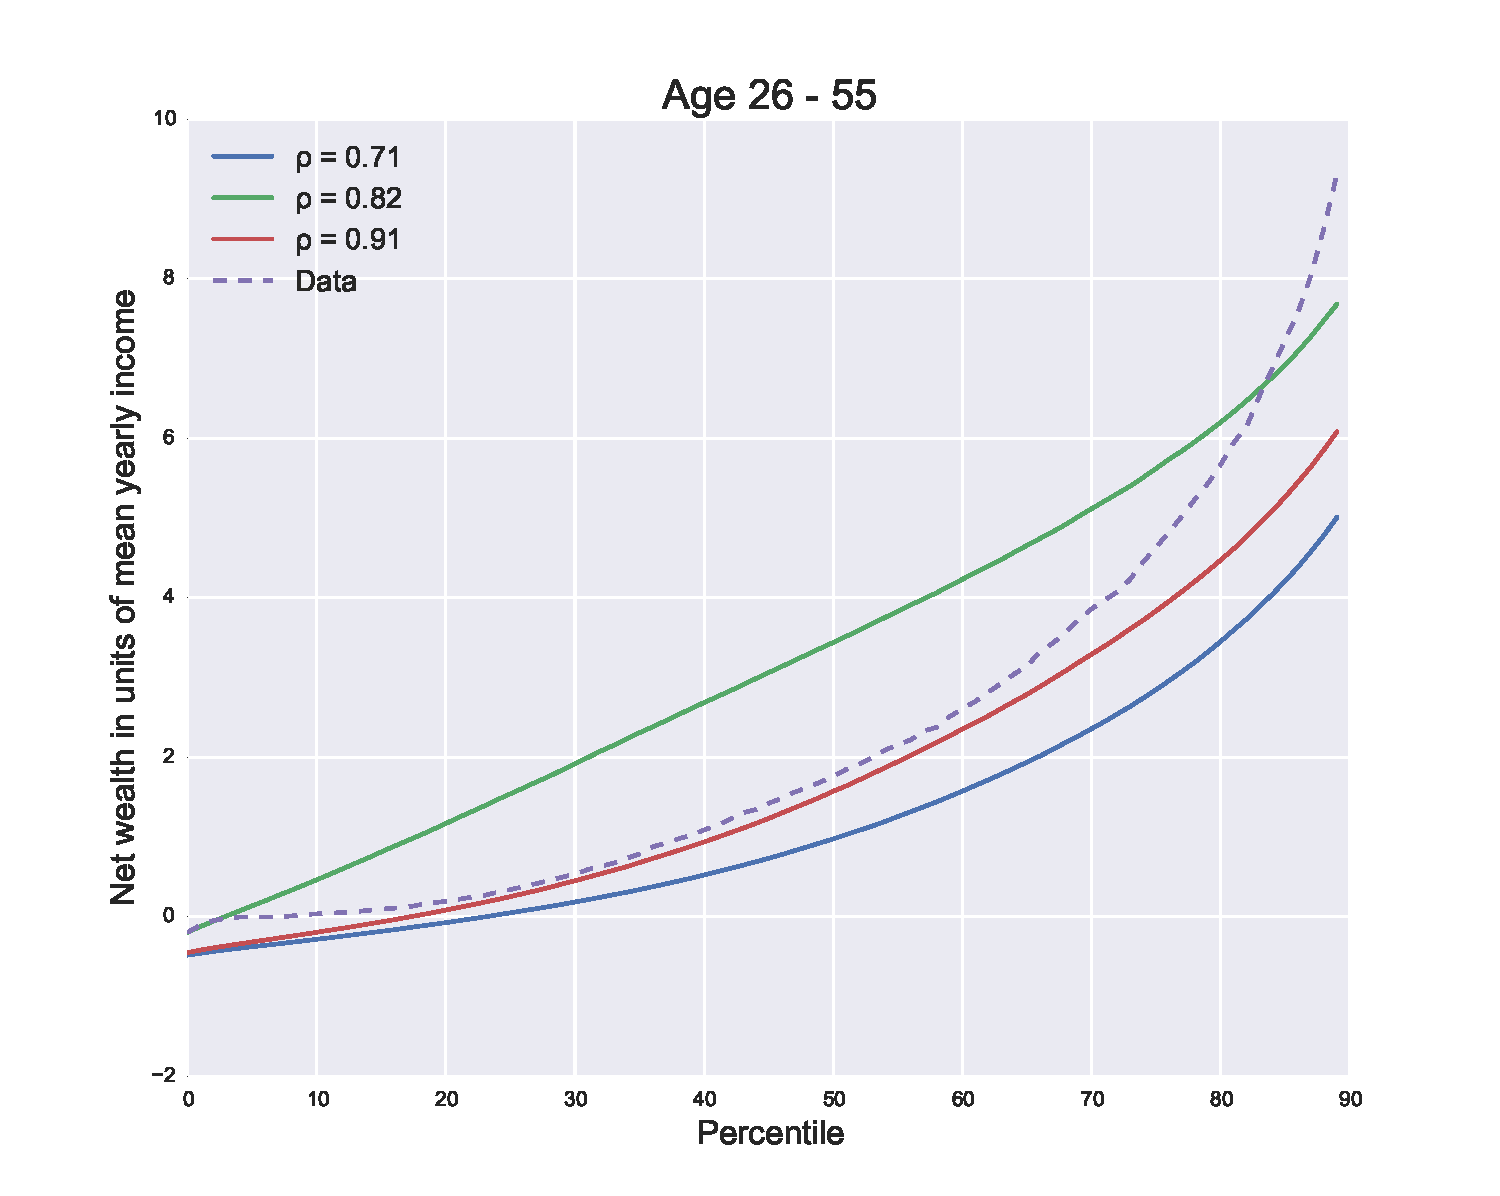
\includegraphics[width=\columnwidth]{comp_stat_rho}
\caption{Comparative statics for variance of individual-specific intercepts, prime age}
\label{fig:comp_stat_rho}
\end{figure}

\begin{figure}
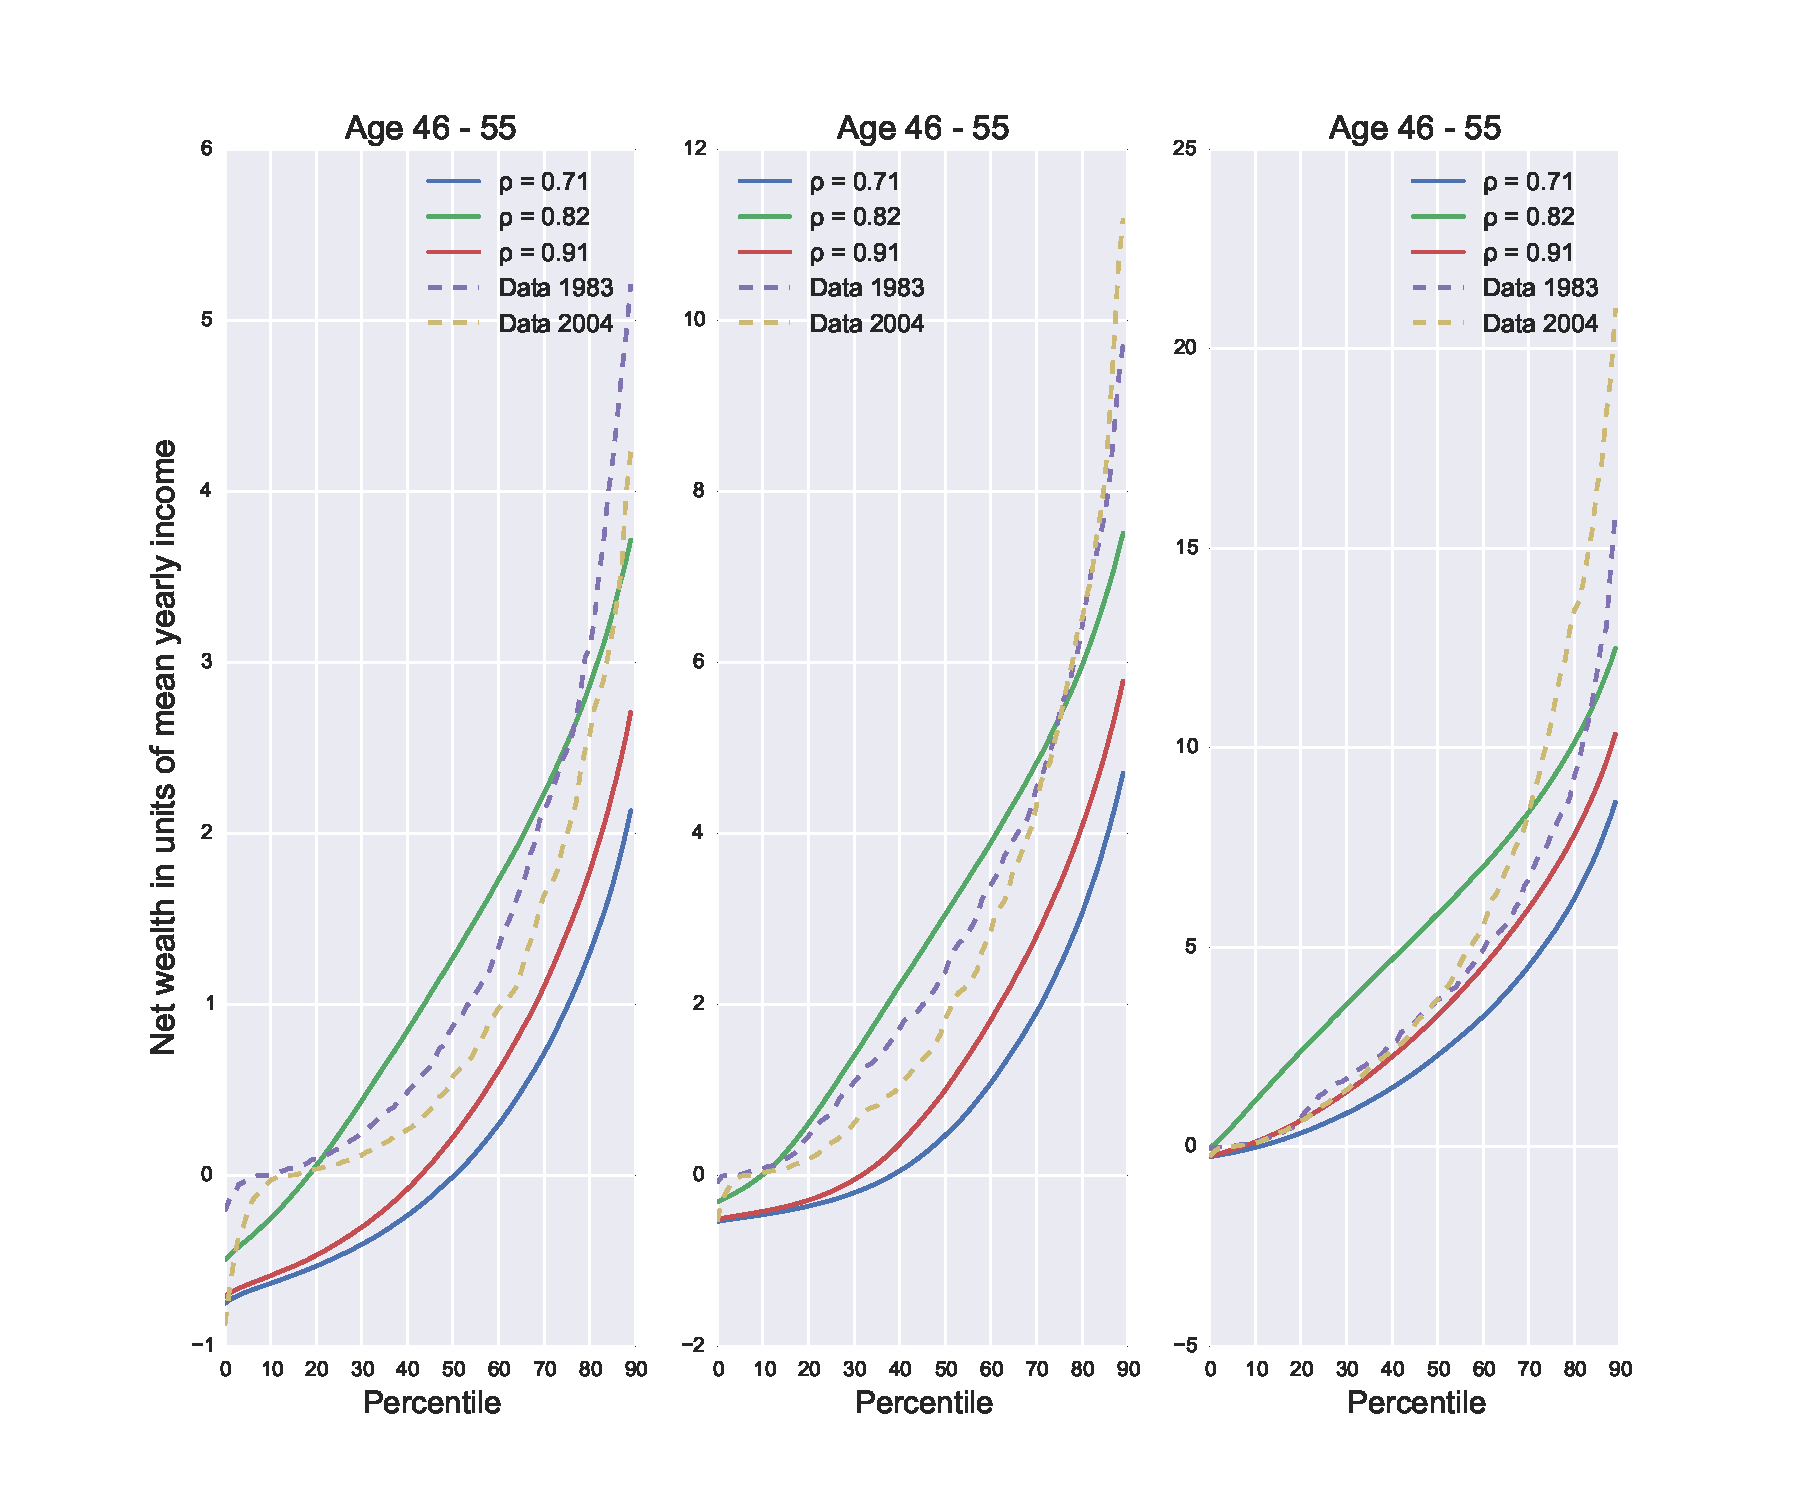
\includegraphics[width=\columnwidth]{comp_stat_rho_agedetail}
\caption{Comparative statics for variance of individual-specific intercepts, by age groups}
\label{fig:comp_stat_rho_agedetail}
\end{figure}

\begin{figure}
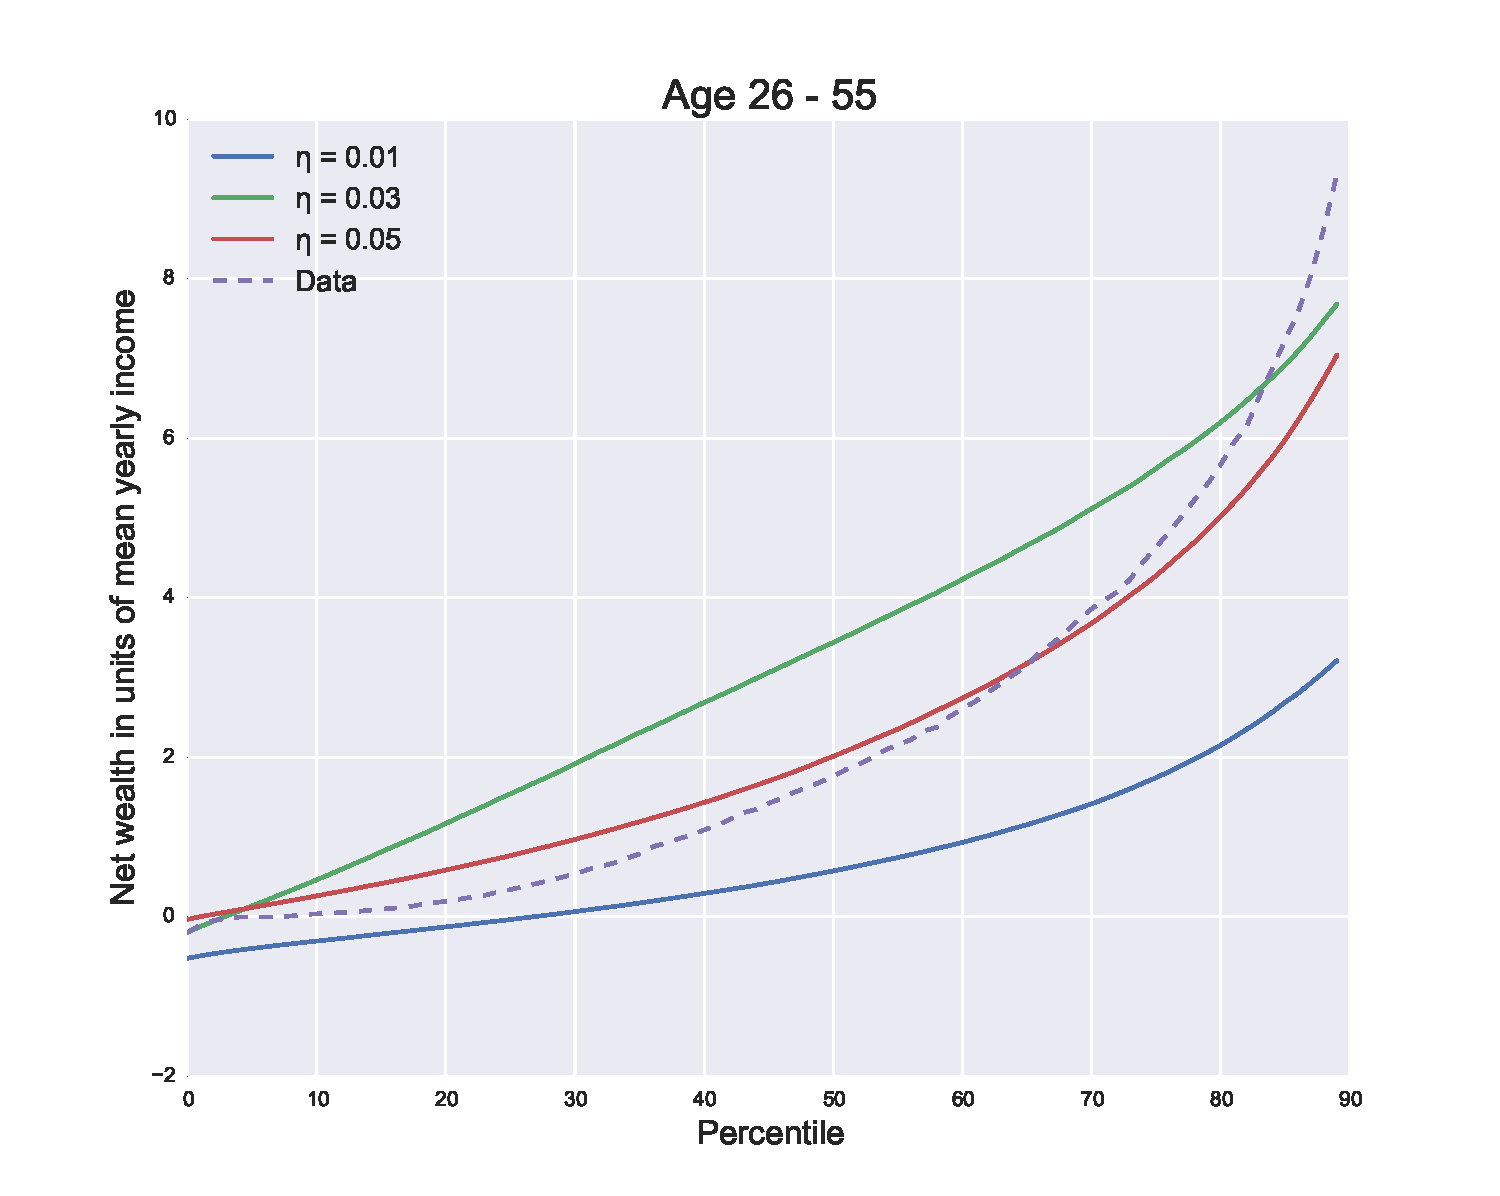
\includegraphics[width=\columnwidth]{comp_stat_eta}
\caption{Comparative statics for variance of individual-specific intercepts, prime age}
\label{fig:comp_stat_eta}
\end{figure}

\begin{figure}
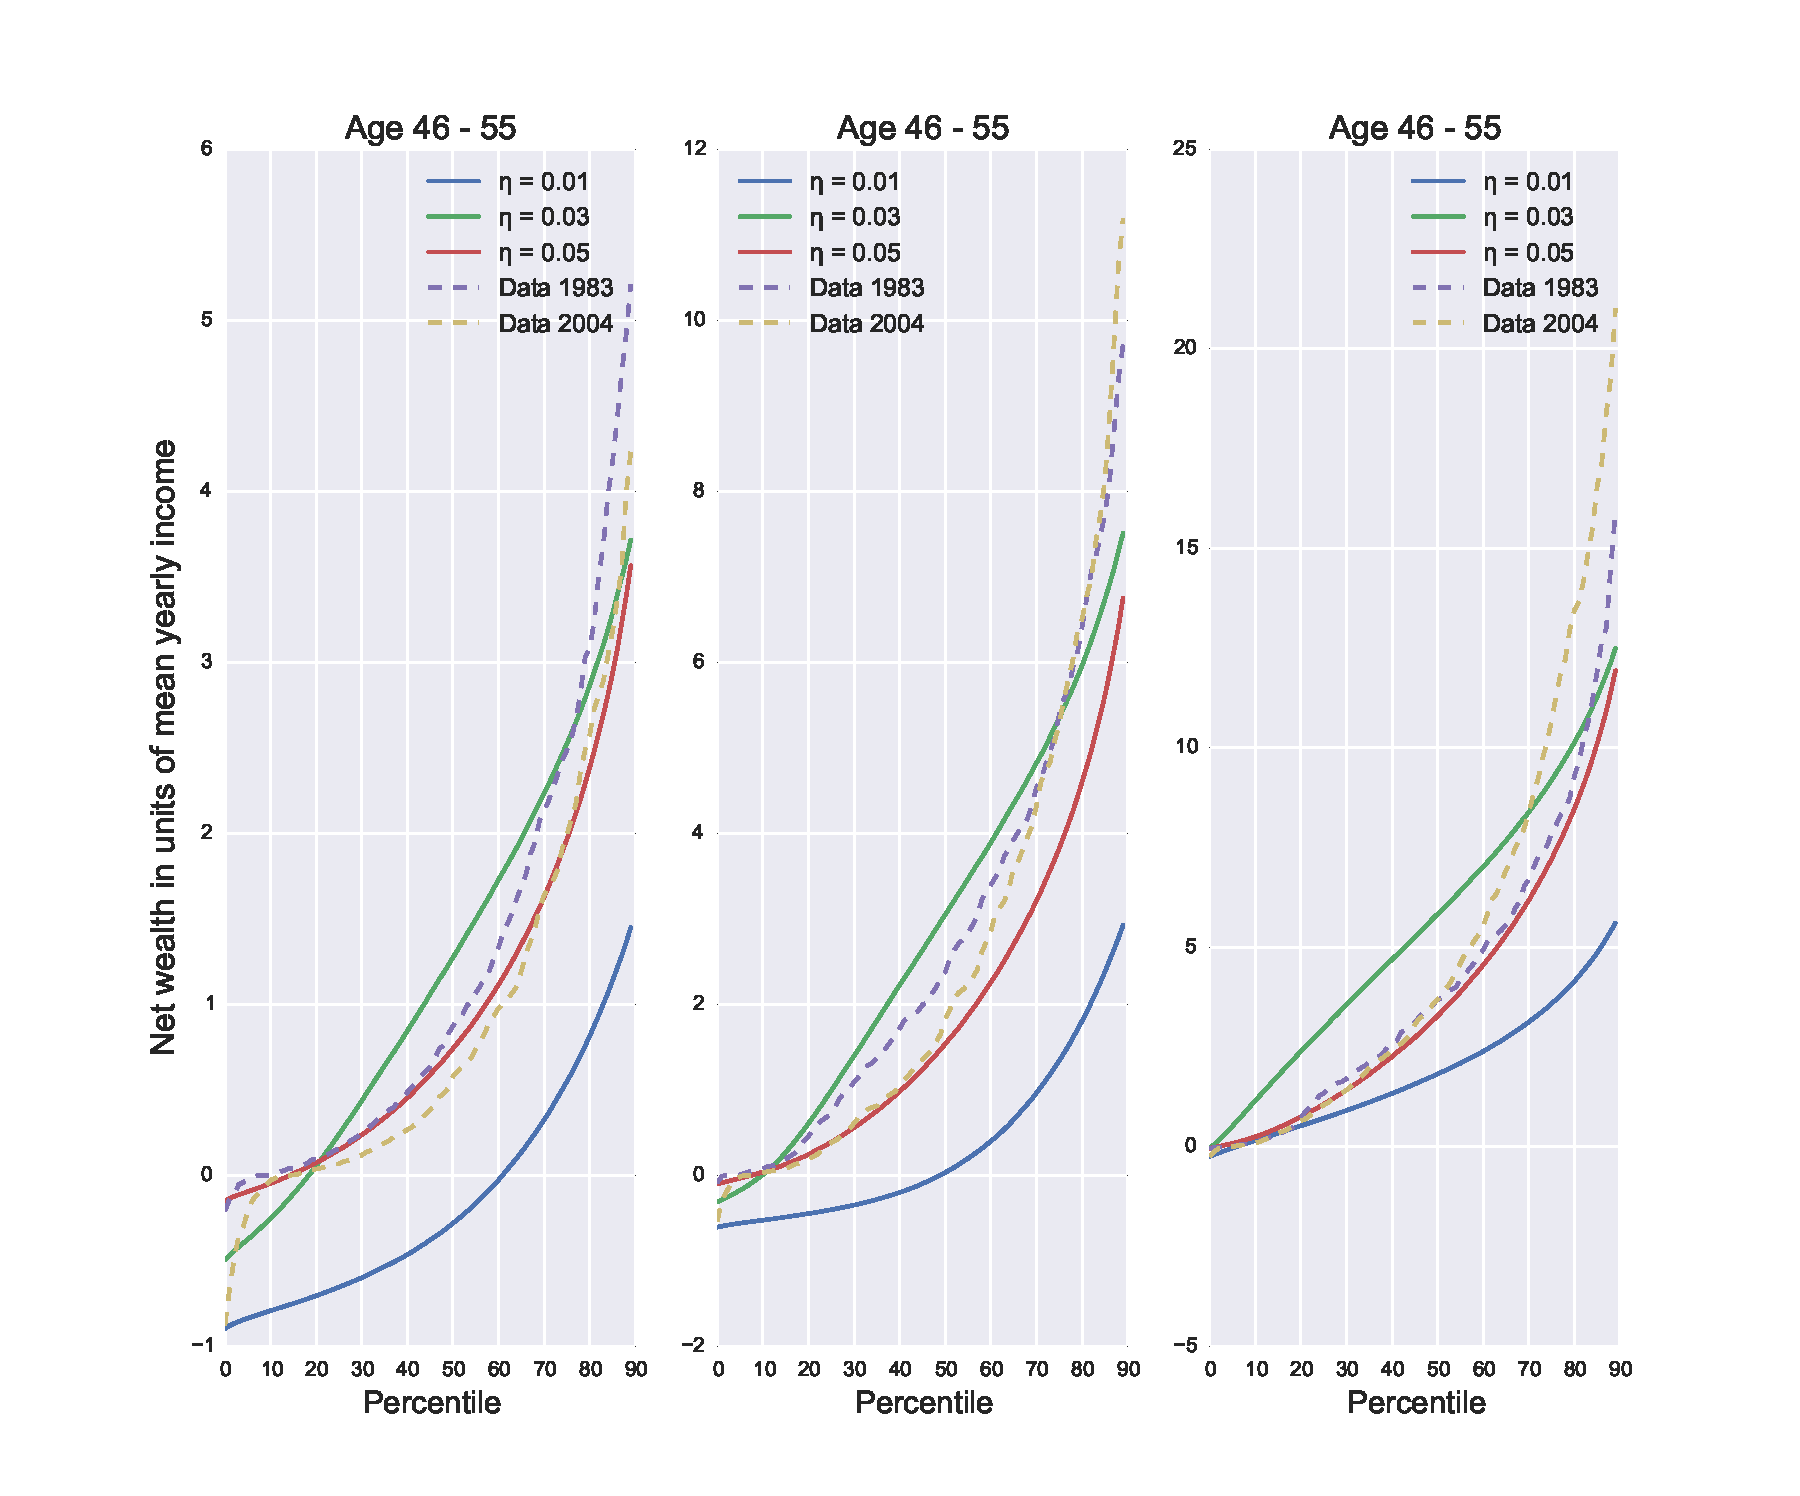
\includegraphics[width=\columnwidth]{comp_stat_eta_agedetail}
\caption{Comparative statics for variance of individual-specific intercepts, by age groups}
\label{fig:comp_stat_eta_agedetail}
\end{figure}

\begin{figure}
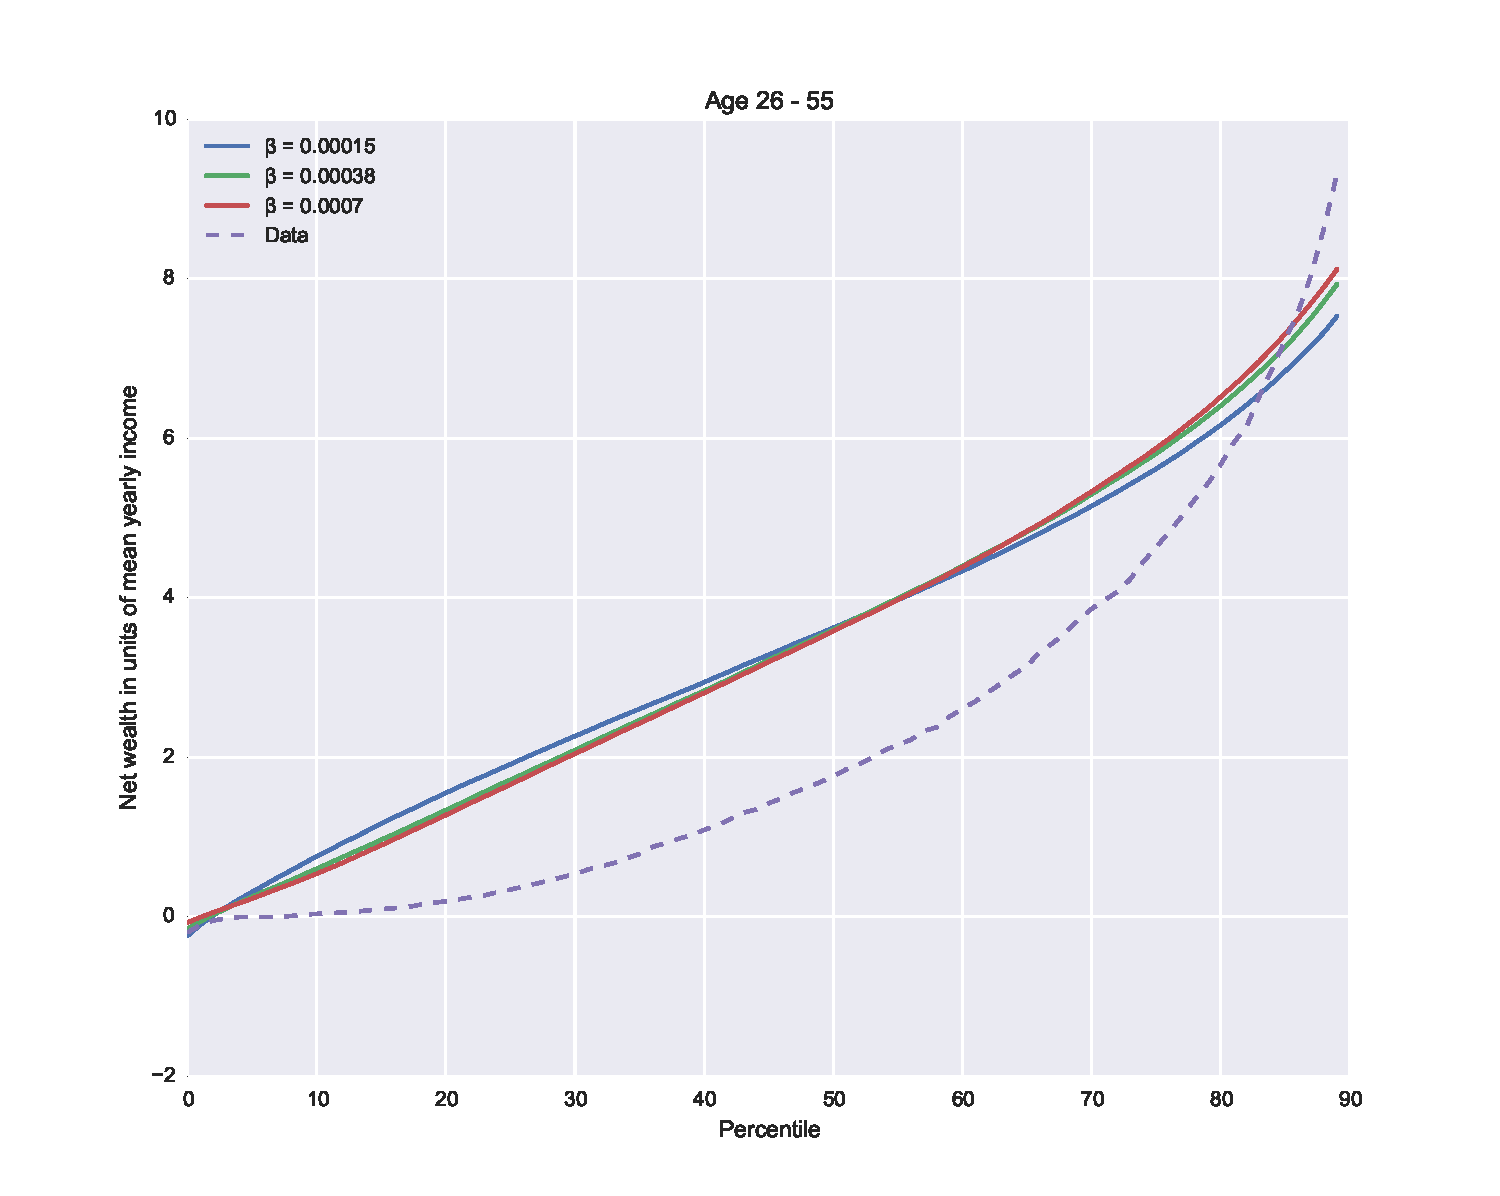
\includegraphics[width=\columnwidth]{comp_stat_beta}
\caption{Comparative statics for variance of individual-specific growth rates, prime age}
\label{fig:comp_stat_beta}
\end{figure}

\begin{figure}
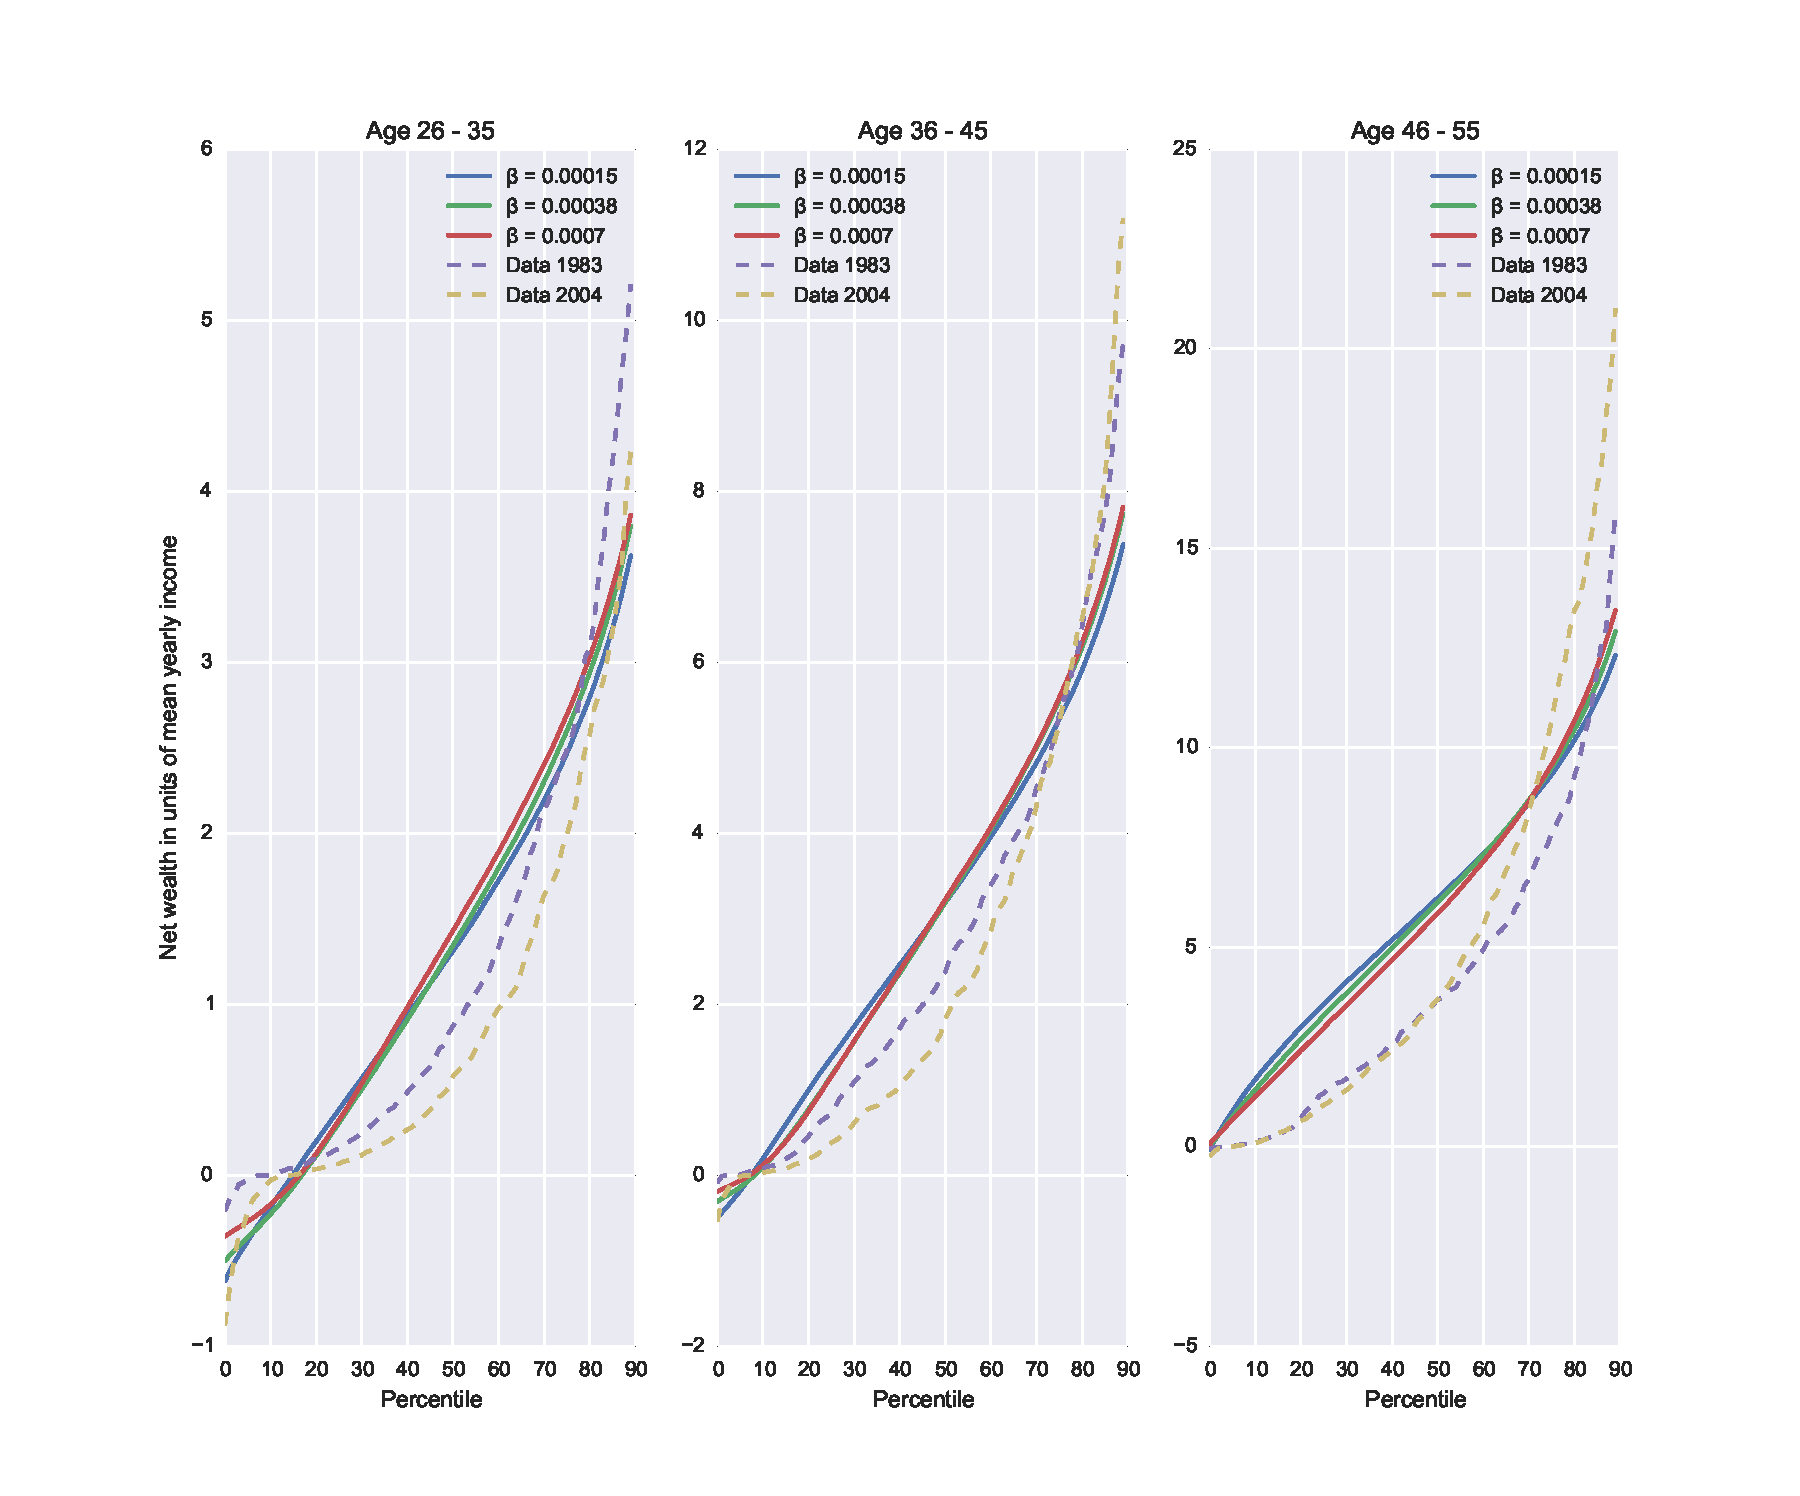
\includegraphics[width=\columnwidth]{comp_stat_beta_agedetail}
\caption{Comparative statics for variance of individual-specific growth rates, by age groups}
\label{fig:comp_stat_beta_agedetail}
\end{figure}


\section{The role of initial beliefs}
One question when working with beliefs is obviously how initial beliefs are 
derived. While the model so far had agents starting with random beliefs centred
around their individual-specific true parameter, and we have discussed the role
of uncertainty induced by learning, we will now briefly consider situations in 
which the initial beliefs are systematically incorrect. Of course, with an 
appropriately chosen set of initial beliefs, the model can be made to produce 
almost any desired result, so that we will only consider two situations which 
are at least supported by anecdotal evidence. The first very simple experiment
is done under the assumption that agents suffer from overconfidence regarding
their own economic fortune. There are a host of studies that offer support for 
the view that people are too optimistic about their future earnings potential,
e.g. a Gallup poll by \citet{Moore2003} in which half of all respondents aged
18 to 29 state that they regard it very or at least somewhat likely to be rich
in the future, with the median figure for expected yearly income and wealth cited at
\$120,000 and \$1 million, respectively. Of course it is questionable whether 
actual economic choices would be based on a vague belief about the indefinite 
future\footnote{Another constraint on this is that these beliefs would require
large amounts of borrowing in the present, for which optimistic people would have
to find lenders who share their beliefs.}, we can use our model to assess what 
would happen if people would indeed act on them. Figure \ref{fig:optimisticbeta}
shows the wealth distribution that obtains if all agents start with a belief 
that is one percentage point above their original initial belief. As expected,
the entire wealth distribution is shifted down

The second scenario under consideration is related to the shifts in the US 
income distribution happening throughout the 80s and 90s. As has been well documented,
wage inequality experienced a secular rise during this period, with top incomes
surging, while incomes at the bottom of the distribution saw their growth rates
fall. To the extent that these changes were unobserved by agents contemporaneously,
and happened through changes in the idiosyncratic growth rates, they might have
biased beliefs of agents entering the labour market, if they form their beliefs
based on past observations of income growth for people in similar places in the 
wealth distribution. To capture a stylised version of this process in the model
we will solve the model assuming that those agents in the upper quintile of the 
true distribution of $\beta$
start life with a belief one percentage point below their original initial belief,
those in percentiles 60 to 80 half a percentage point lower, those in percentiles
20 to 40 half a percentage point higher, and those in the bottom quintile one 
percentage point higher. The results in figure \ref{fig:wrongbetabelief} show 
a tilting of the wealth distribution, with agents at the upper end accumulating
more wealth, since they ascribe a larger part of their good fortune to permanent
shocks given that they systematically underestimate their deterministic growth
rate. At the same time, more agents at the lower end of the distribution are 
constrained, as they expect higher future income growth than will actually 
materialise. These changes in the wealth distribution are consistent with the
observed increase in wealth inequality that followed the increase in income 
inequality in the 1980s and 90s (as discussed in \citet{Iacoviello2008}) and 
could form the basis of a demand-driven expansion of household debt at the lower
end of the income distribution. Indeed, rising income inequality is often cited as 
a prime reason for the increase in household indebtedness (see e.g. \citet{Rajan2011},
\citet{SaezZucman2014}, or, for a more heterodox treatment, \citet{BarbaPivetti2009}),
although from the standpoint of a standard life-cycle model of consumption and 
savings this link should be absent, given that recent work based on Social 
Security records shows virtually the entire increase in income inequality to
be due to permanent, rather than transitory shocks, which should result in 
changes in consumption, rather than wealth inequality. One possibility for 
permanent changes in the income distribution not to immediately filter through
to the consumption distribution could then, according to our model, be hysteresis
in belief formation of agents entering the labour market at different points
of the income distribution.

\begin{figure}%
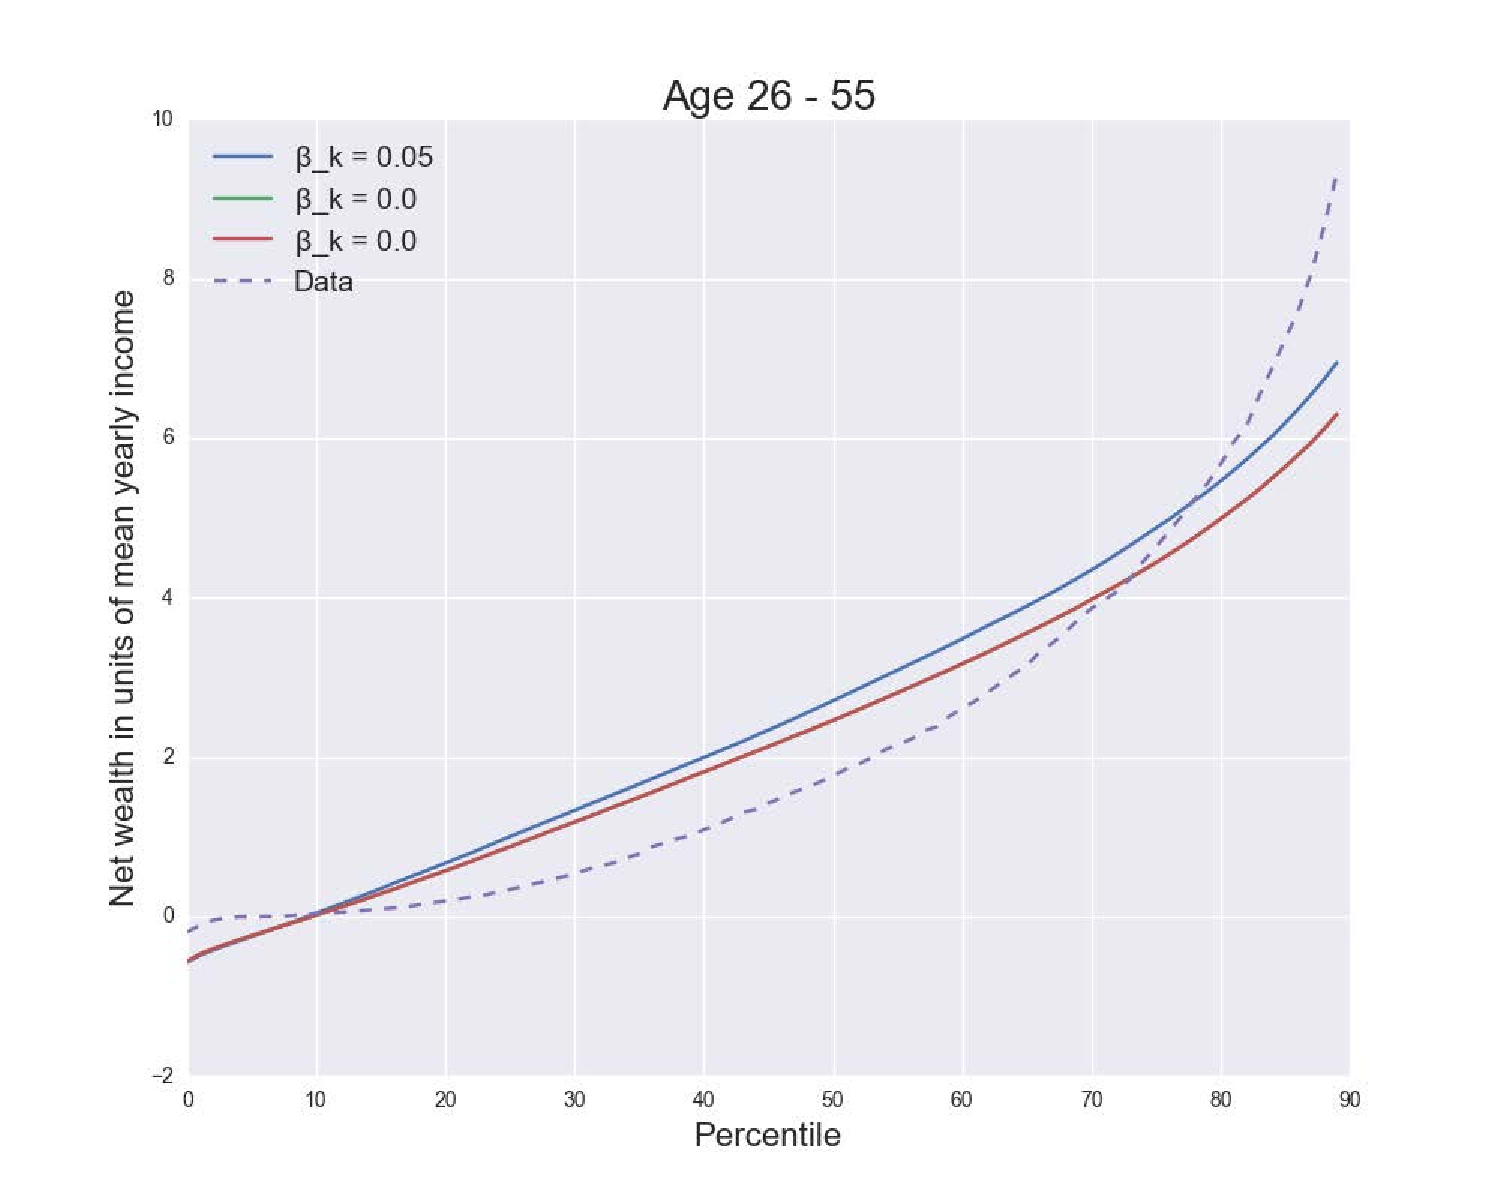
\includegraphics[width=\columnwidth]{optimisticbeta}%
\caption{Effects of incorrect initial beliefs}%
\label{fig:optimisticbeta}%
\end{figure}


\begin{figure}%
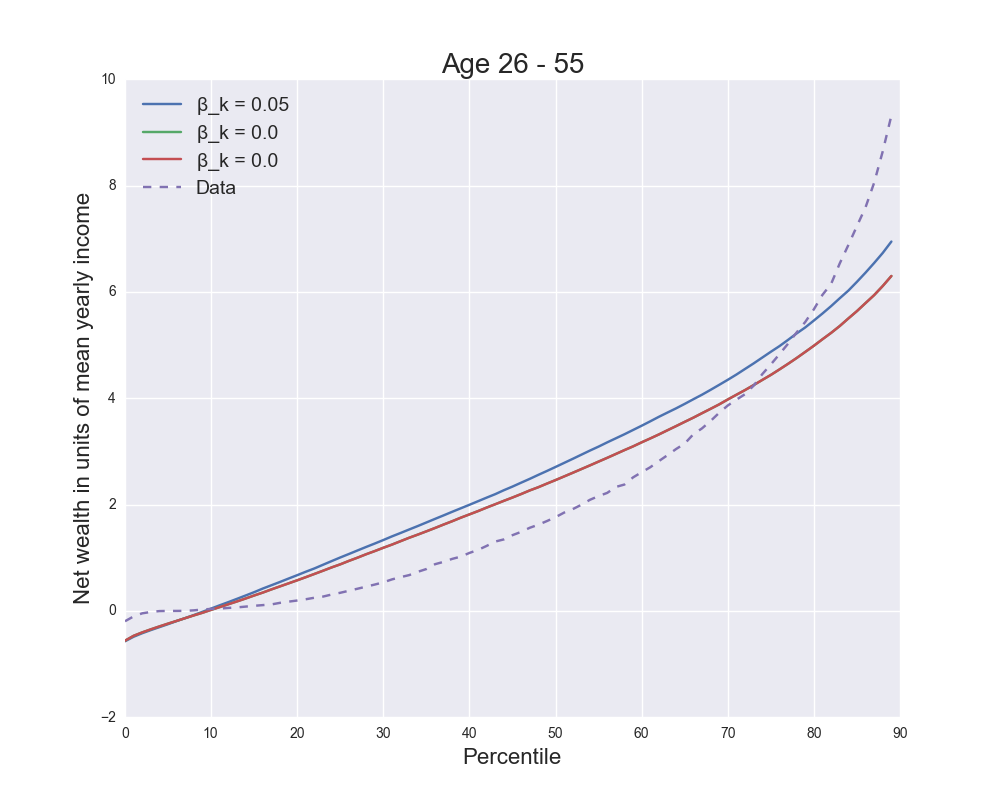
\includegraphics[width=\columnwidth]{wrongbetabelief}%
\caption{Effects of incorrect initial beliefs}%
\label{fig:wrongbetabeliefs}%
\end{figure}


\section{Discussion}\label{sec:discussion}
As this chapter has shown, the learning model of heterogeneous income processes
fails in capturing the dynamics of the wealth distribution under all calibrations
derived from empirical data on income processes. Comparing the model output of 
different counterfactual parametrisations, it became clear that the main reason
behind this is not the learning mechanism itself, but the different income 
distribution and risk implied by the heterogeneous income process. To salvage 
the model, ad-hoc changes to the belief structure of agents can be made, although
at this point it becomes a bit of a free-for-all and the model can be made to
predict any pattern in the data with a suitable choice of initial beliefs.
Building on the work in this chapter, future research should consider the implications
of other more realistic income processes on the wealth distribution, to the 
extent that they can be formulated parsimoniously enough not to increase the 
computational burden beyond reason. An example would be the work by 
\citet{MeghirPistaferri2004}, who model the conditional variance of income
shocks using an ARCH model and show analytically that the addition of individual-
specific heterogeneity in the innovation variance leads to both a larger dispersion
of savings rates and higher aggregate saving. A further case of interest would be
the specification derived by \citet{GKOS2015}, which adapts the income process
used in this chapter by adding two more AR(1) components with different innovation
variances, so that households are subject to potential shocks of different 
magnitude. As the evidence points to this process being the best description 
of the income risk households are facing in reality, the implications of this
process for the wealth distribution should be investigated further. 

\section{Appendix A: Comparative statics results}

\begin{figure}
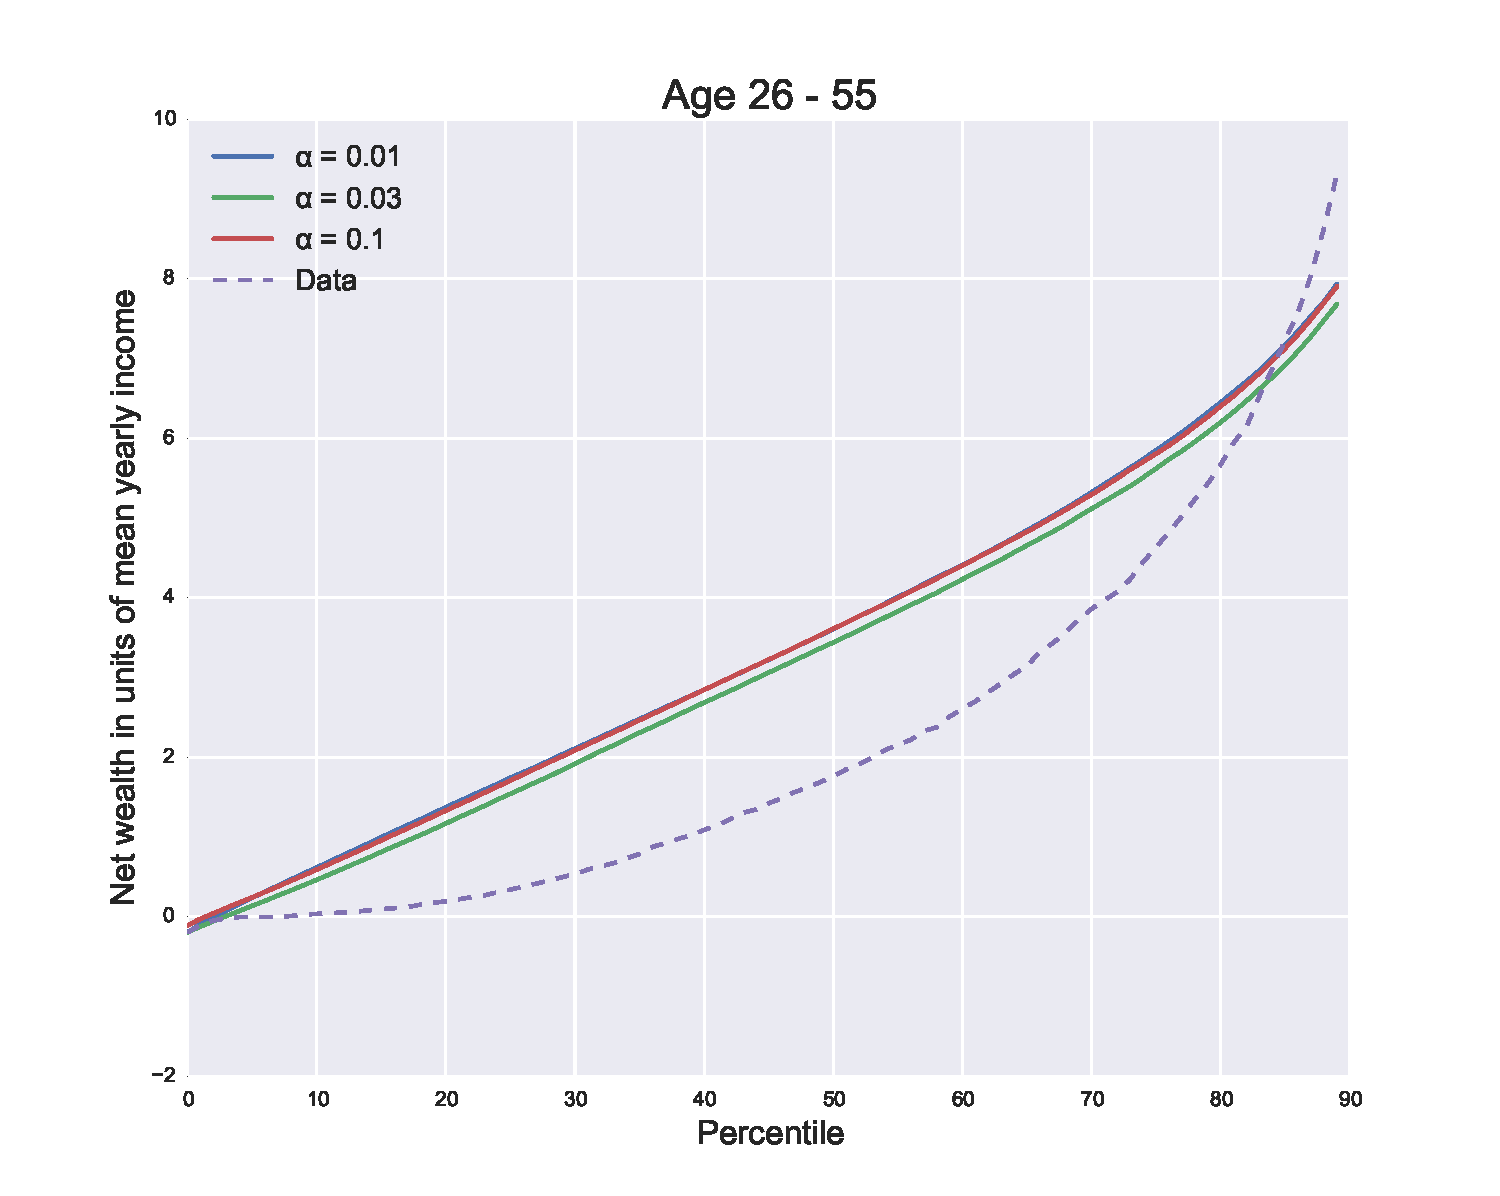
\includegraphics[width=\columnwidth]{comp_stat_alpha}
\caption{Comparative statics for variance of individual-specific intercepts, prime age}
\label{fig:comp_stat_alpha}
\end{figure}

\begin{figure}
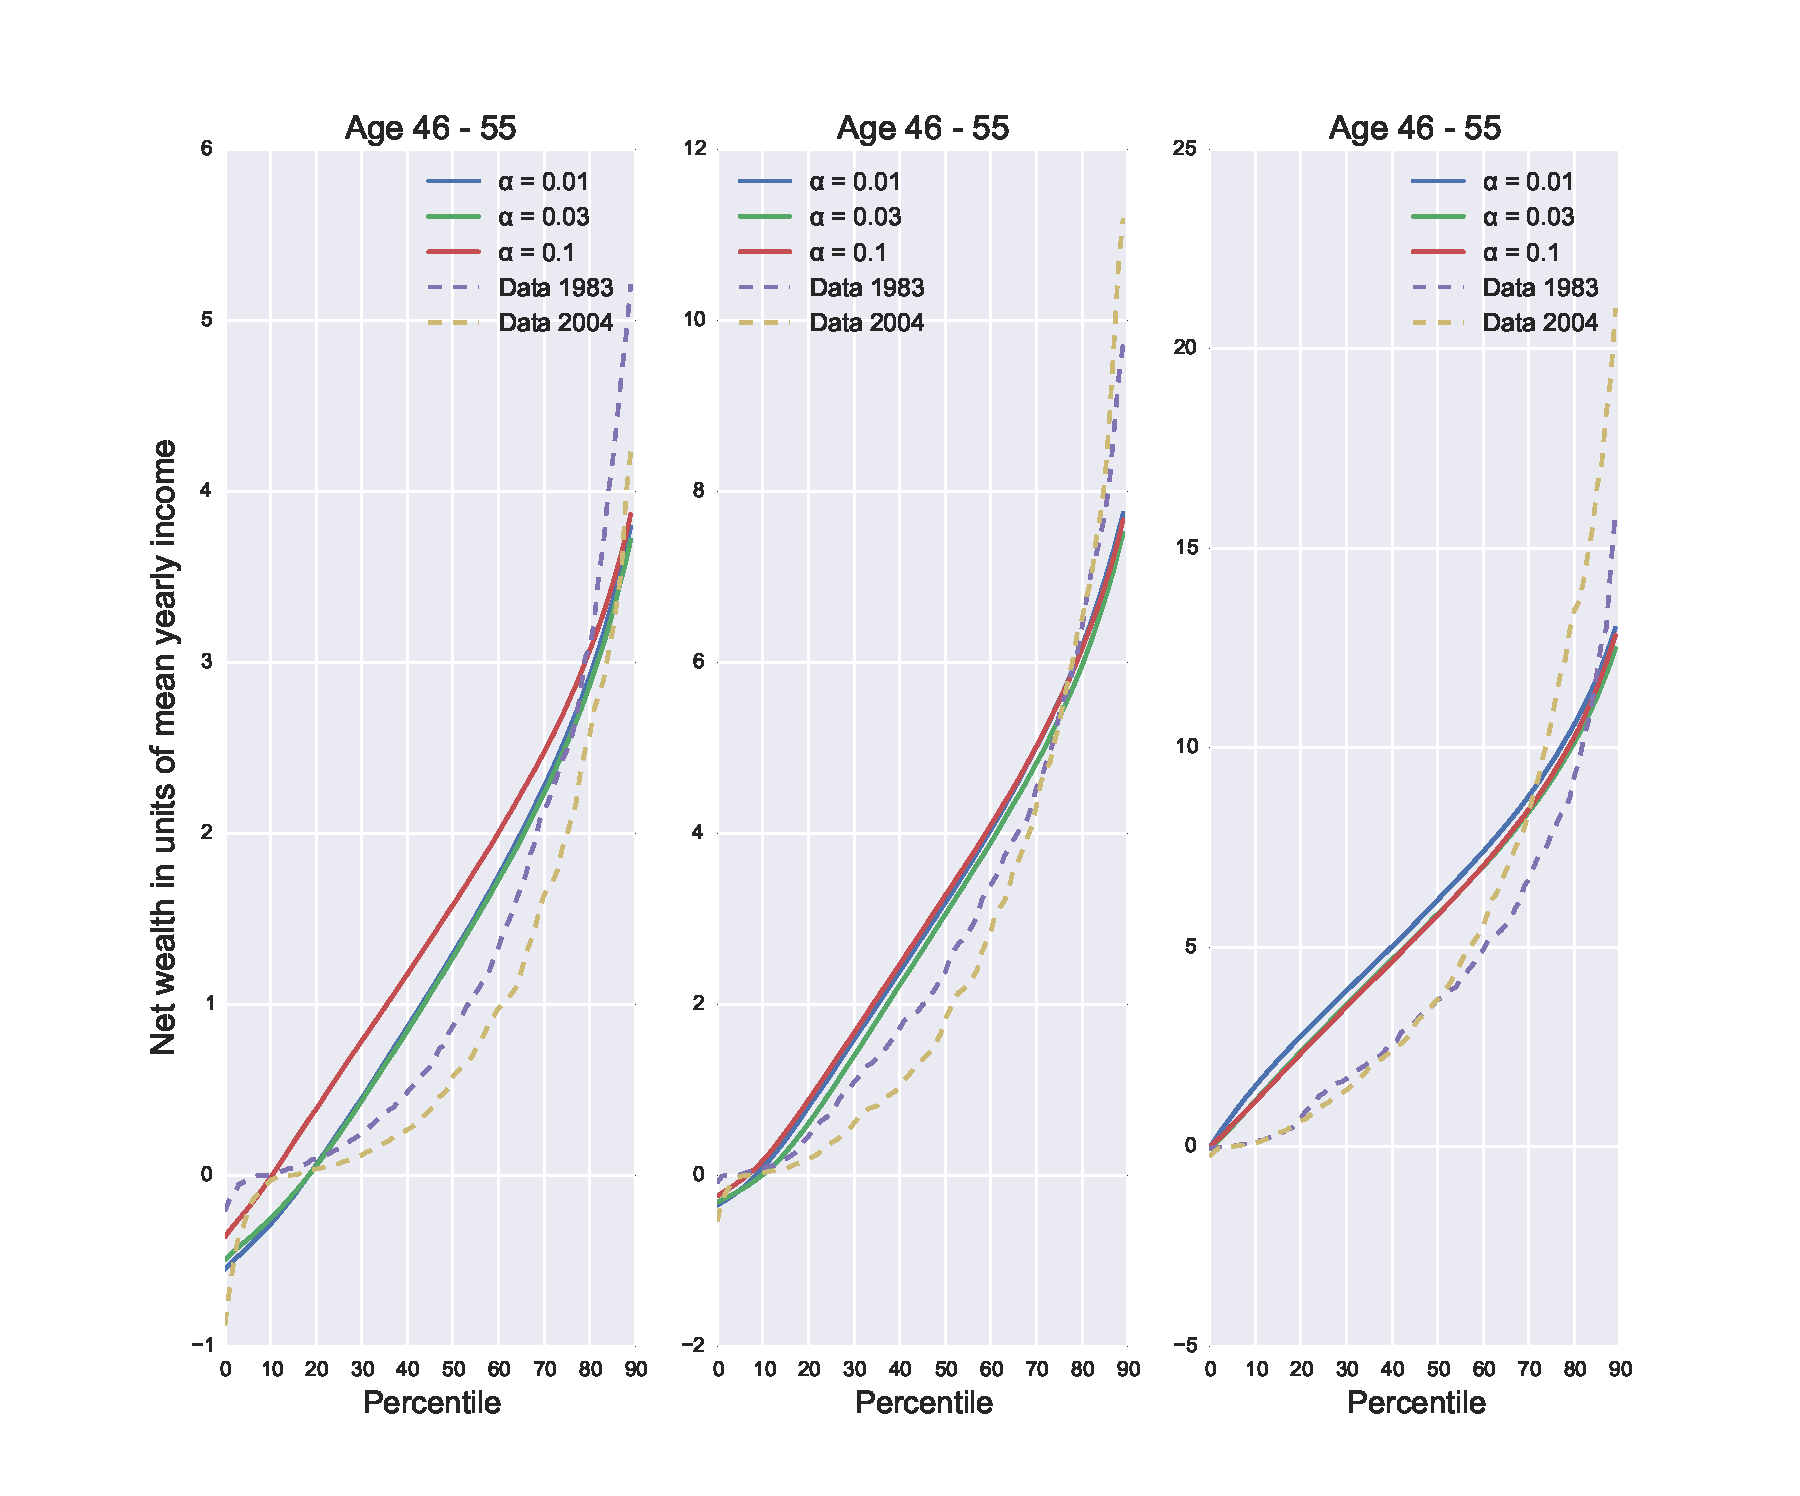
\includegraphics[width=\columnwidth]{comp_stat_alpha_agedetail}
\caption{Comparative statics for variance of individual-specific intercepts, by age group}
\label{fig:comp_stat_alpha_agedetail}
\end{figure}

\begin{figure}
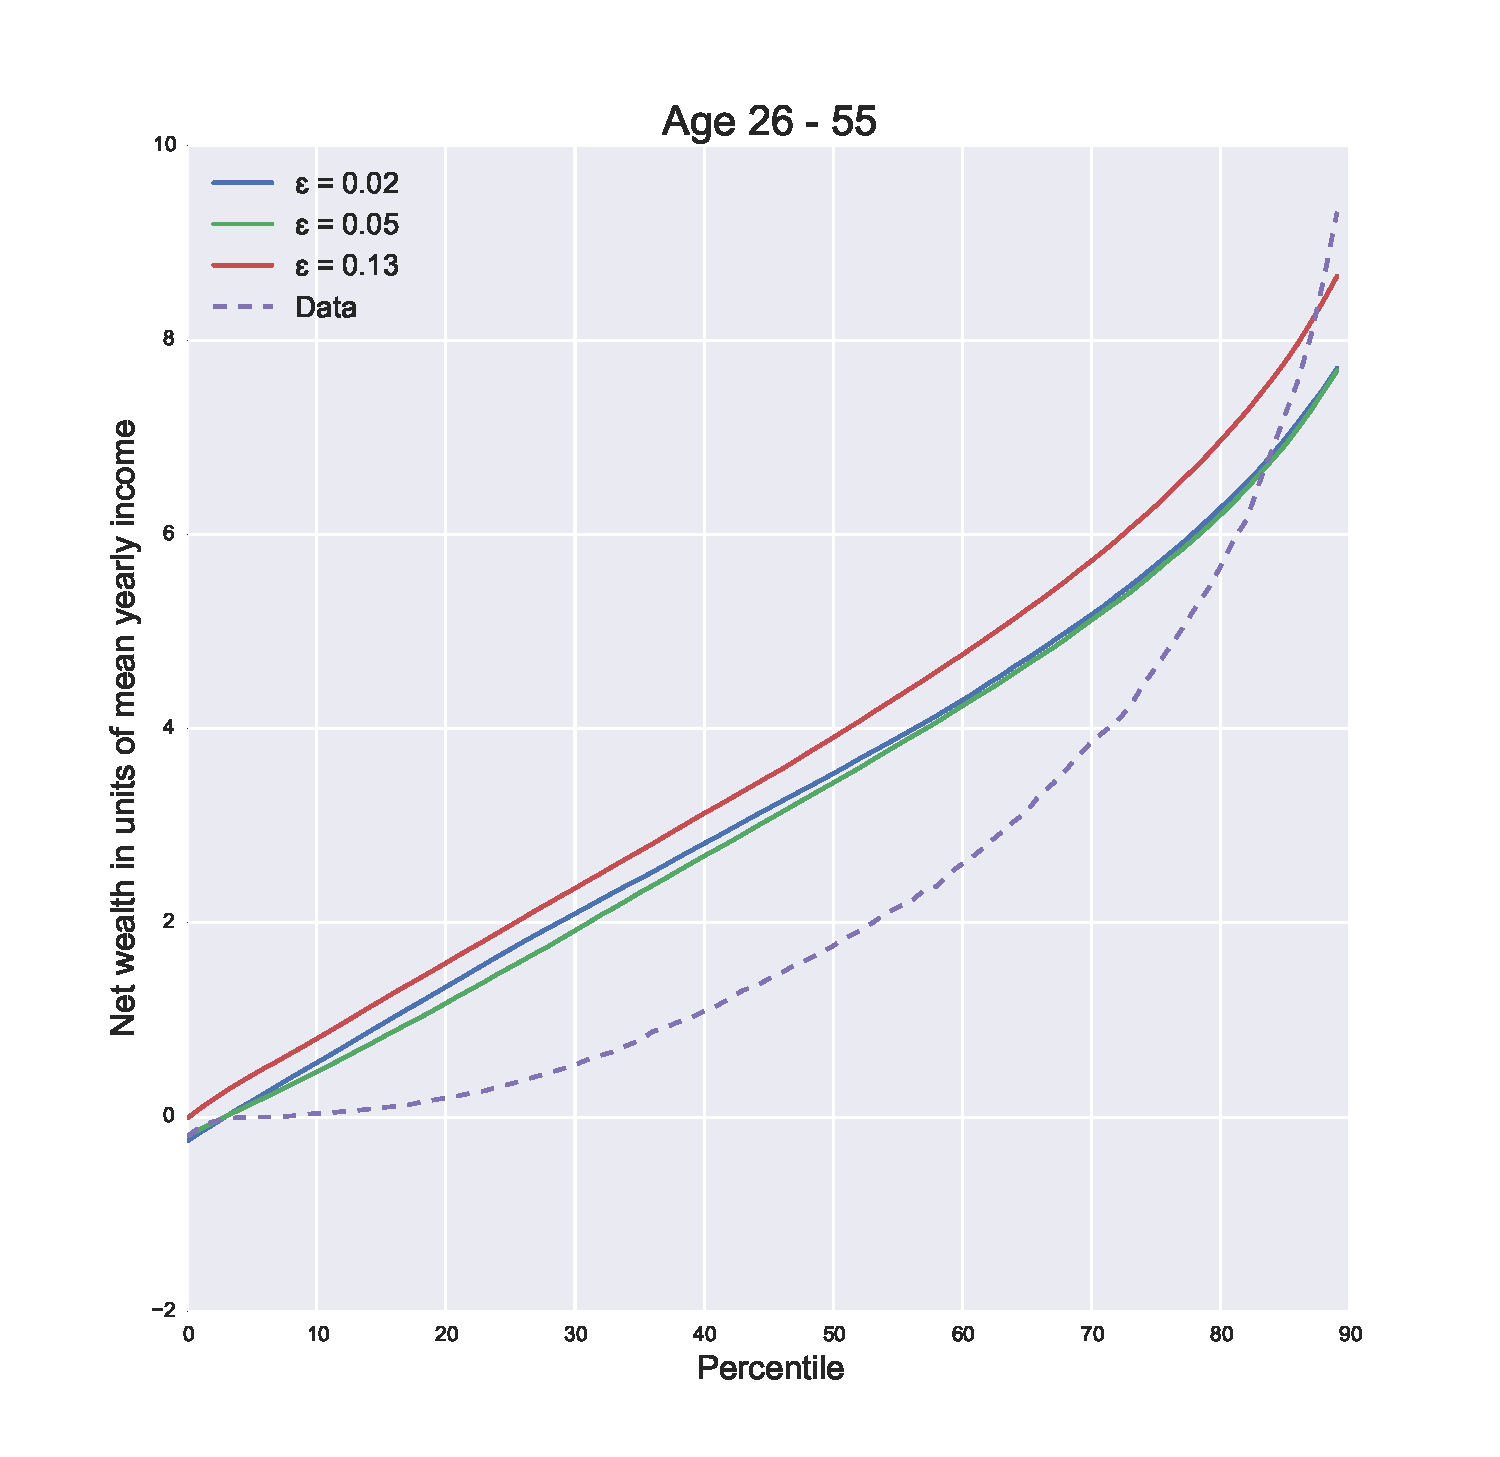
\includegraphics[width=\columnwidth]{comp_stat_eps}
\caption{Comparative statics for variance of transitory shocks, prime age}
\label{fig:comp_stat_eps}
\end{figure}

\begin{figure}
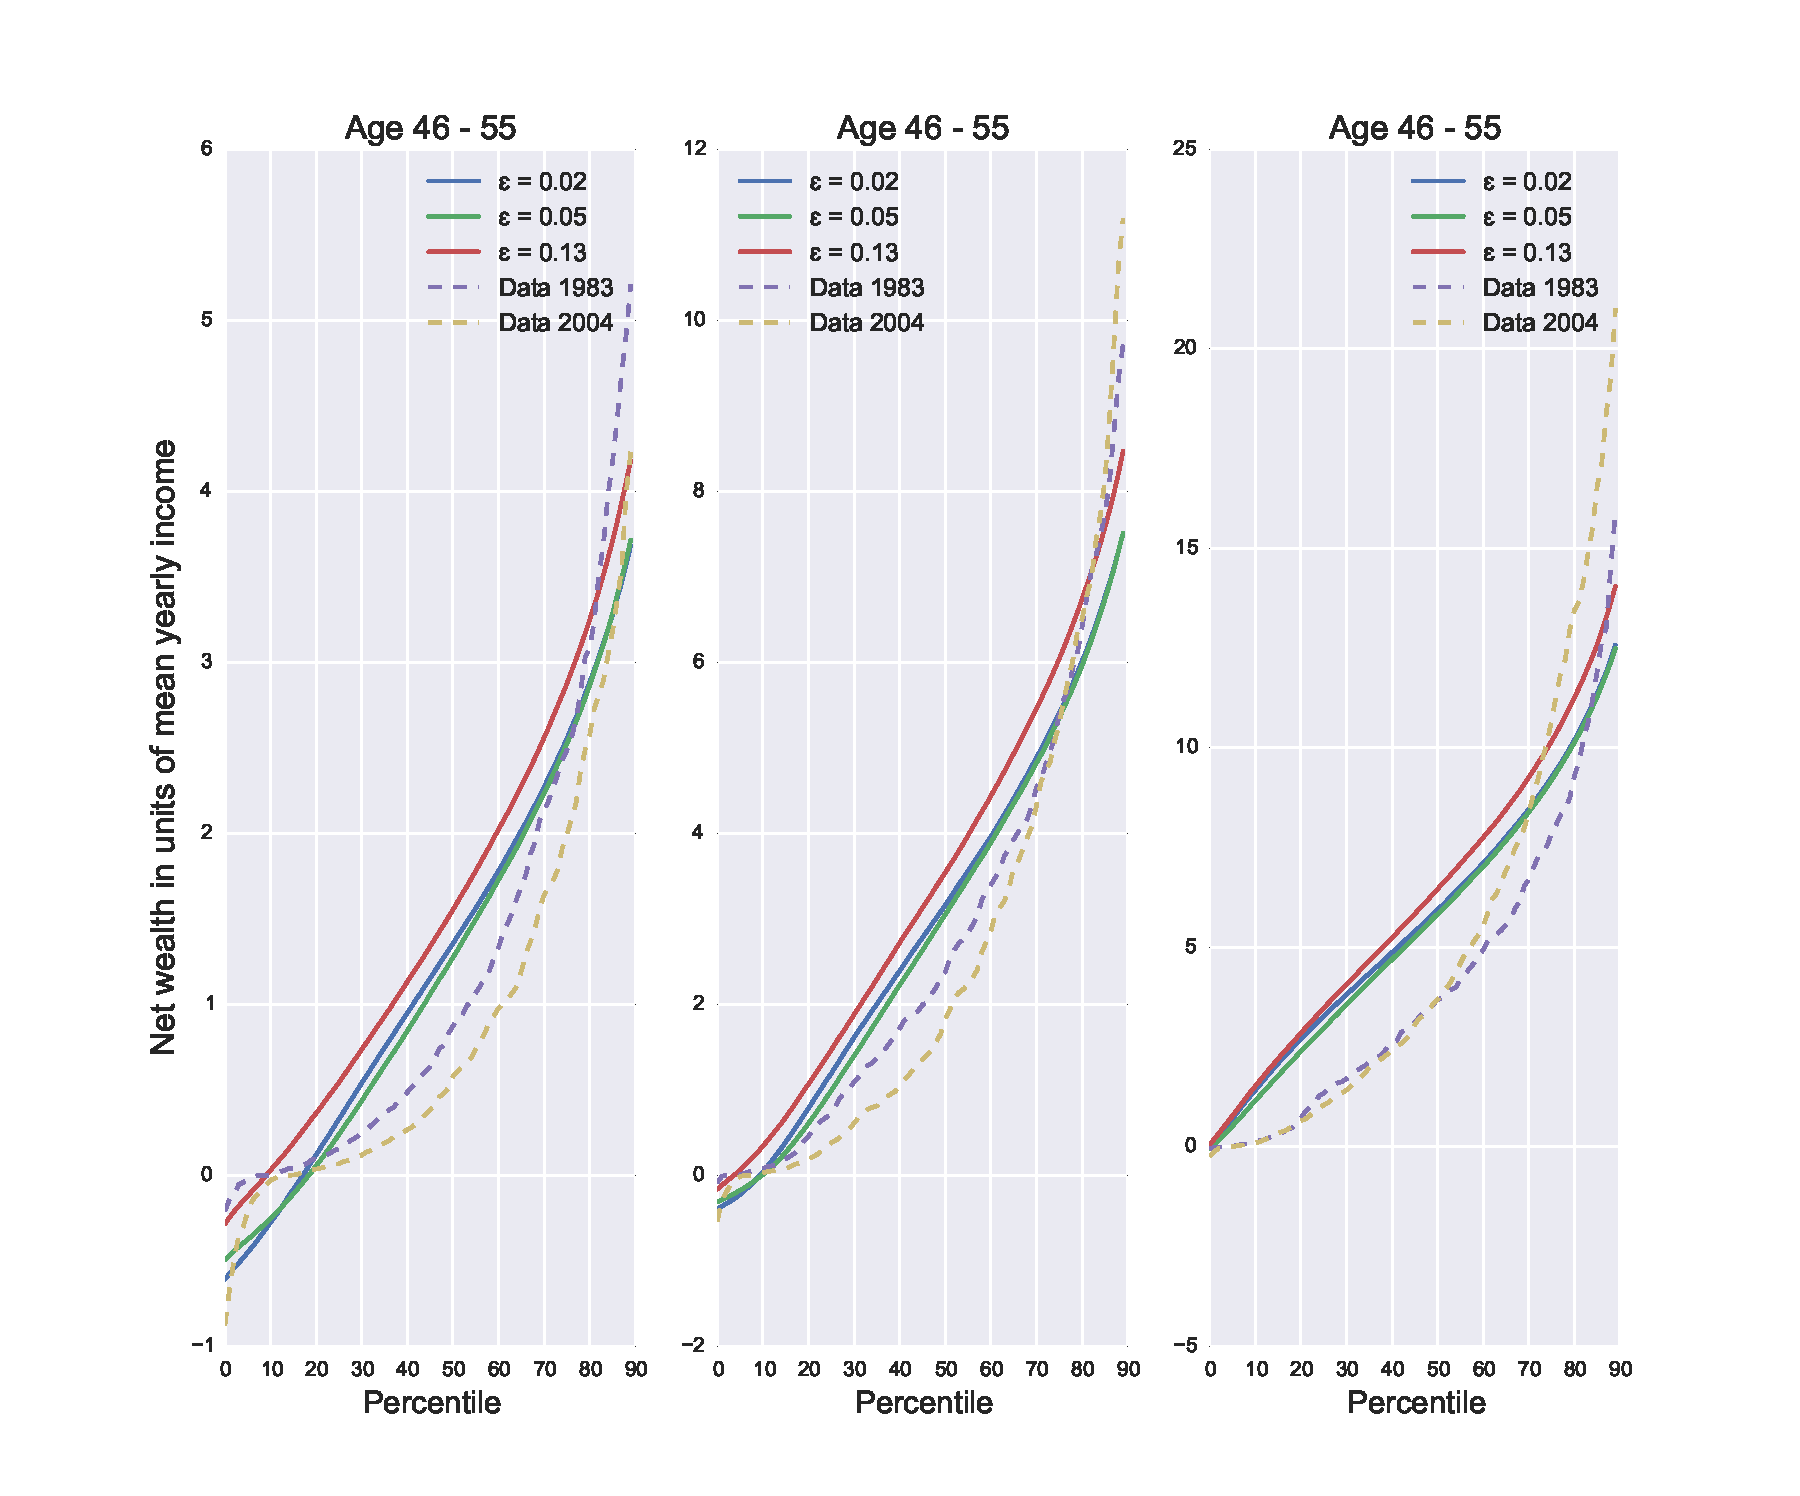
\includegraphics[width=\columnwidth]{comp_stat_eps_agedetail}
\caption{Comparative statics for variance of transitory shocks, by age group}
\label{fig:comp_stat_eps_agedetail}
\end{figure}

\begin{figure}
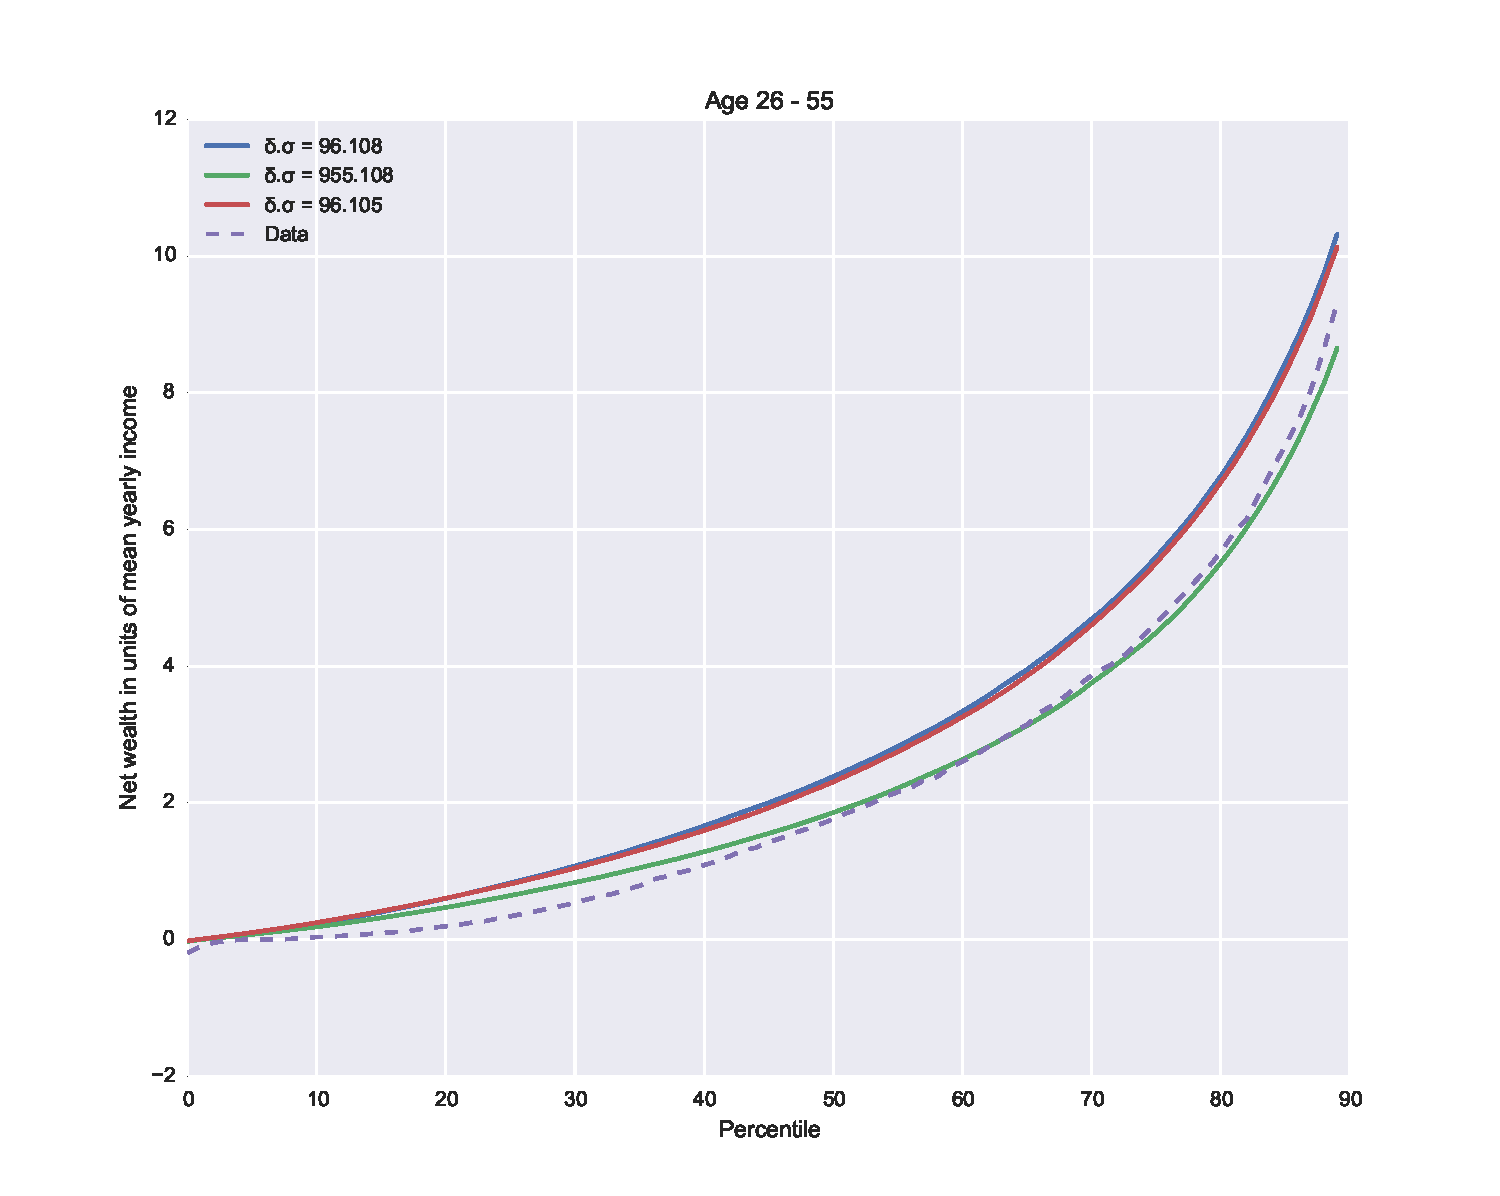
\includegraphics[width=\columnwidth]{winfriedcompare}
\caption{Model fit when income is an RIP process with $\rho=0.95$ and $\sigma^2_{\eta}=0.5$}
\label{fig:winfriedcompare}
\end{figure}

\begin{figure}
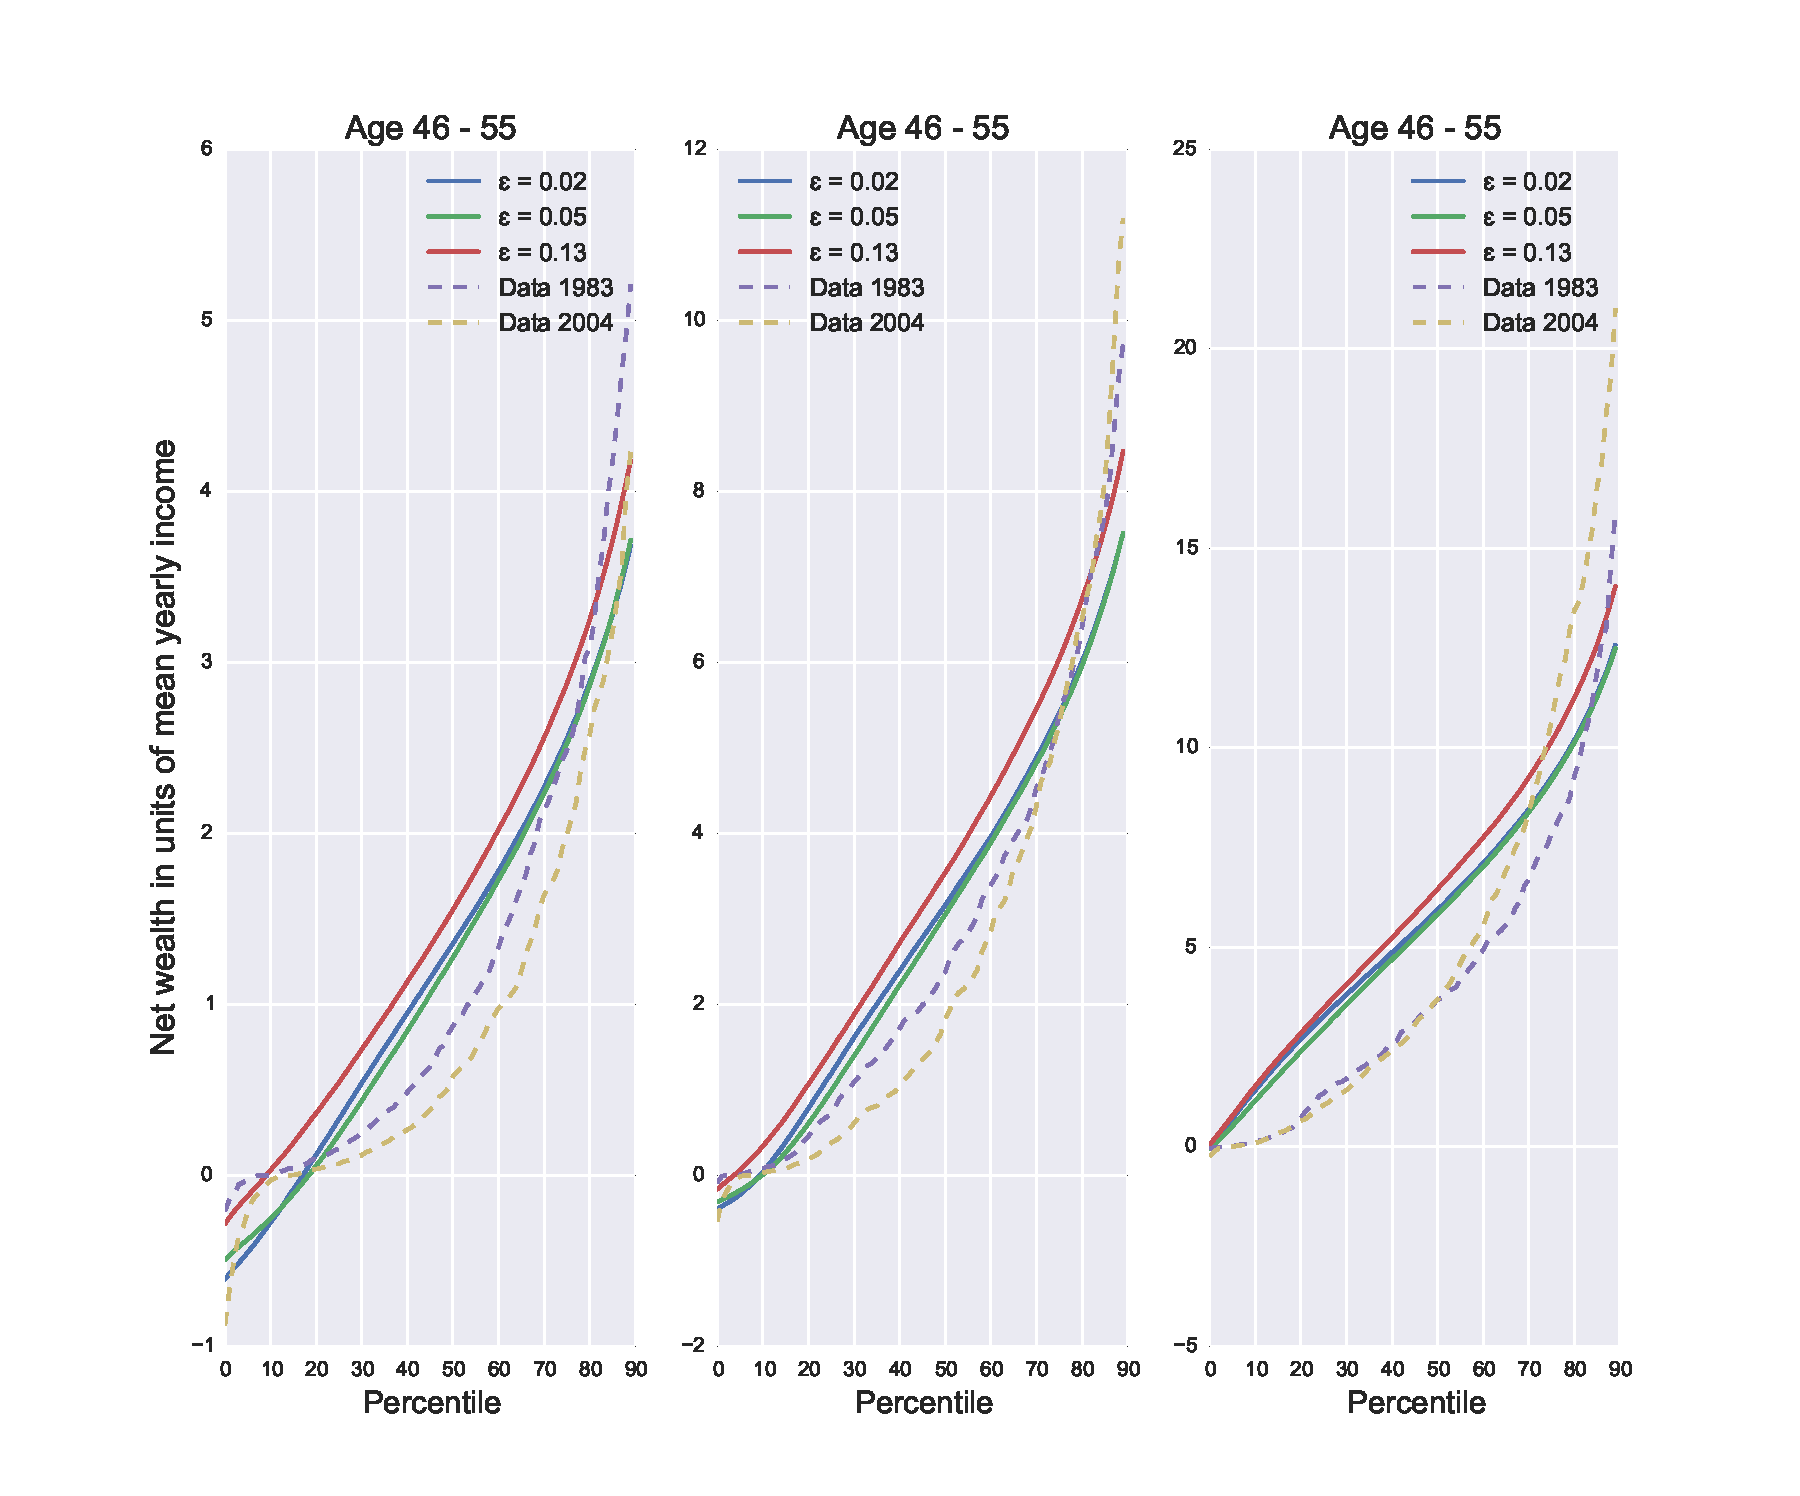
\includegraphics[width=\columnwidth]{comp_stat_eps_agedetail}
\caption{Model fit when income is an RIP process with $\rho=0.95$ and $\sigma^2_{\eta}=0.5$, by age groups}
\label{fig:winfriedcompare_agedetail}
\end{figure}

\begin{figure}
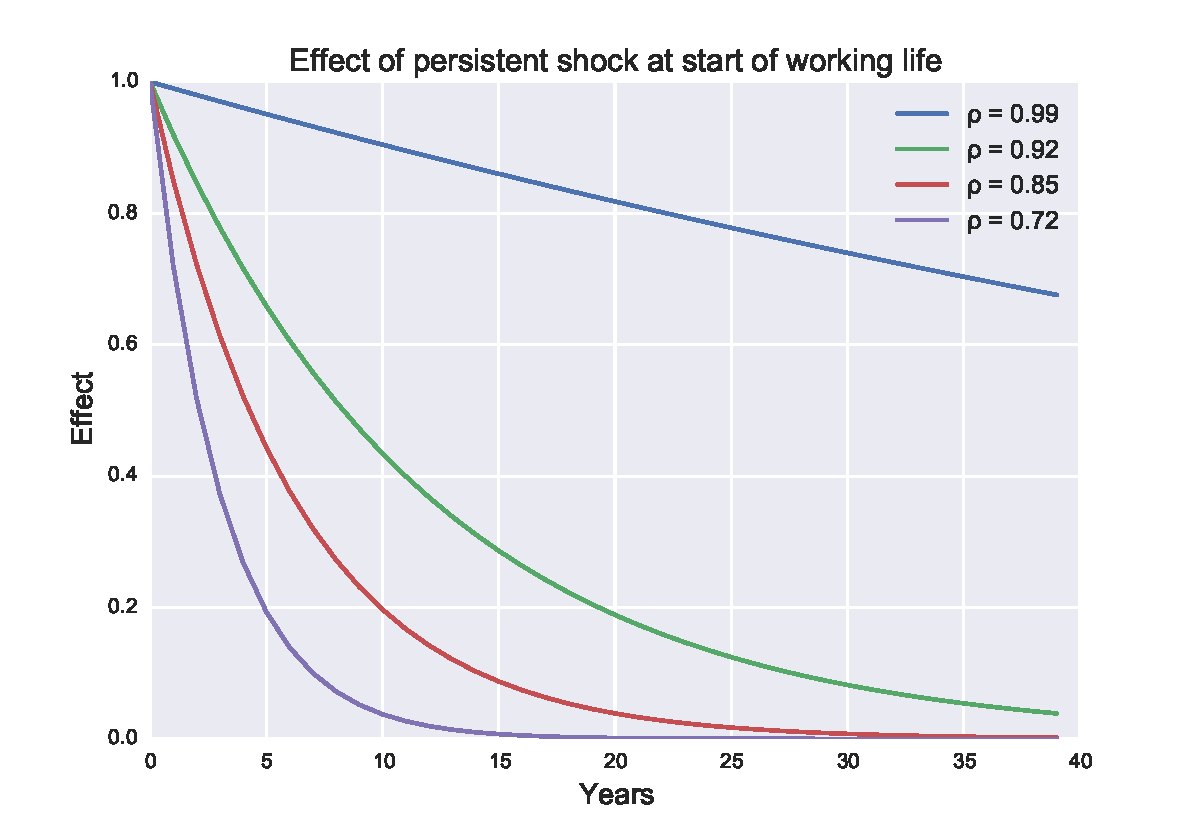
\includegraphics[width=\columnwidth]{effect_rho}
\caption{Effects of lowering $\rho$ on half life of persistent shocks}
\label{fig:effect_rho}
\end{figure}